\documentclass[11pt,openany]{book}
\usepackage{graphicx}
\usepackage{amssymb}
\usepackage{color}

\textwidth = 7 in
\textheight = 9 in
\oddsidemargin = -0.3 in
\evensidemargin = -0.3 in
\topmargin = -0.25 in
\headheight = 0.0 in
\headsep = 0.5 in
\parskip = 0.1in
\parindent = 0.0in


% this is based on the C2.8 rev 3 manual
%
% Copyright 2011, Range Networks, Inc.
% Do no not redistribute without permission.
%


\date{}
\renewcommand{\familydefault}{\sfdefault}

\title{
\textsf{

\includegraphics[width=\textwidth]{RangeLogo.pdf} \vspace{0.25in}
{\Huge \textbf{OpenBTS P2.8}} \\ 
Users' Manual \\  \vspace{0.25in}
%\emph{Working Draft} \\ \vspace{1in}
Doc.~Rev.~3  \\
\vspace{1.5in}
This document is licensed under a Creative Commons Attribution-ShareAlike 3.0 Unported License.}
}


\begin{document}
\maketitle

\tableofcontents
\listoffigures
\listoftables

\chapter{Introduction}
The OpenBTS P2.8 ``Opelousas'' release is distributed publicly under the AGPLv3 license.
P2.8 provides the following improvements over previous the P2.6 AGPLv3 ``Mamou'' public release:
\begin{itemize}
	\item External configuration control and status reporting through an sqlite3 database file.
	\item Syslogd support.
	\item In-call delivery and submission of text messages.
	\item Support for binary payloads and non-Latin alphabets in SMS.
	\item RRLP.
	\item Standalone subscriber registry database and ``realtime'' Asterisk support.
	\item Many bug-fixes in the SIP and call control modules.
	\item Support for new types of digital radio hardware, beyond the Ettus USRP1:
	\begin{itemize}
		\item Ettus USRP2
		\item Range Networks RAD1 and Leapfrog devices
	\end{itemize}
\end{itemize}

The P2.8 release is derived from the C2.8 commercial release.%
\footnote{There is no P2.7 release; the C2.7 ``Natchitoches'' commercial release had no corresponding public release.}
The C2.8 release has the same architecture as P2.8, but includes the following additional features:
\begin{itemize}
	\item Emergency call support, with priority channel allocation and optional IMS headers.
	\item SMSCB.
	\item Multi-ARFCN operation.
	\item A3/A8 authentication based on a SIP challenge-response exchange.
\end{itemize}
For more information about products based on commercial releases of OpenBTS, see Section~\ref{sec:contact}.
\section{Scope and Audience}
This document describes the organization and operation of the OpenBTS P2.8-series GSM access point software.  It is intended for use by software developers.

\section{Disclaimers}

\subsection{Warranty}
The OpenBTS software and its associated documentation are provided with NO WARRANTY OF ANY KIND.  

Although the information in this handbook has been carefully checked for accuracy, and is believed to be correct and current, no warranty, either express or implied, is made as to either its applicability to, or its compatibility with, specific requirements; nor does Range Networks, Inc.\ assume any responsibility for correctness of this information, nor for damages consequent to its use. All design characteristics and specifications are subject to change without notice.

Range Networks, Inc.\ welcomes any reports of software failures or documentation errors and will make reasonable efforts to correct these in future releases.

\subsection{Accuracy}
This manual is a description of the OpenBTS software, not a specification.
In any discrepancy between the software and this manual, the software source code is authoritative.

\subsection{Patent Laws}
OpenBTS P2.8 is distributed for educational and experimental purposes.
The use of this software to provide GSM services may result in the use of
patented technologies.  The user of this software is required to take whatever
actions are necessary to avoid patent infringement.

\subsection{Trademarks}
``OpenBTS'' is a registered trademark of Range Networks, Inc. (Range), a US corporation.
Range reserves the right to control the use of this trademark.
Do not use this trademark in commerce without permission and do not rebrand OpenBTS under a different trademark.

``Asterisk'' is a trademark of Digium, Inc.

\subsection{Telecom and Radio Spectrum Laws}
Users of this software are expected to comply with all applicable local, national and international
regulations.

\subsection{Software Licensing and Distribution}
OpenBTS P2.8  is distributed in source code form under APGLv3, protected under copyright law. This software is not ``public domain''.  AGPLv3 is a commercial software license, enforceable like any other.

OpenBTS P2.8 also incorporates other components acquired under GPL-family licenses.

\subsubsection{GPL Compliance}
The following components of OpenBTS P2.8 were acquired under GPL variants and are included in source code form in the AGPLv3 distributions:
\begin{itemize}
	\item URSP interface libraries use in the ``transceiver'' applciation
\end{itemize}

\subsubsection{LGPL Compliance}
The following publicly-available packages are linked dynamically by applications in the OpenBTS P2.8 suite under LGPL licenses:
\begin{itemize}
\item UnixODBC.  Public distribution available from http://www.unixodbc.org/.  License is LGPL v2.1.
\item libosip2.  Public distribution available from http://www.gnu.org/software/osip/.  License is LGPL.
\item libortp.  Public distribution available from http://www.linphone.org/.  License is LGPL v2.1.
\end{itemize}
In each case, OpenBTS uses the public distribution without modification.

\section{Abbreviations}
\begin{itemize}
	\item APDU -- application protocol data unit
	\item ARFCN -- absolute radio frequency channel number
	\item BTS -- base transceiver subsystem
	\item dB -- Decibels
	\item dBm -- Decibel milliwatts
	\item FEC -- forward error correction
	\item GPL -- General Public License
	\item kHz -- kilohertz
	\item LNA -- low-noise amplifier
	\item LGPL -- Lesser General Public License
	\item MOC -- mobile-originated call
	\item MO-SMS -- mobile-originated SMS
	\item MTC -- mobile-terminated call
	\item MT-SMS -- mobile-terminated SMS
	\item MS -- mobile station
	\item PA -- power amplifier
	\item PDU -- protocol data unit
	\item preamp -- low-noise amplifier
	\item RF -- radio frequency
	\item RPDU -- relay-layer protocol data unit
	\item RRLP -- radio resource location protocol
	\item SIP -- Session Initiation Protocol
	\item SMS -- Short Message Service
	\item TDM -- time-division multiplexing
	\item TPDU -- transfer-layer protocol data unit
	\item USSD -- unstructured supplementary service data
	\item VDC -- Volts, direct current
	\item W -- Watts
\end{itemize}


\section{References}

\subsection{ETSI/3GPP}
This document references the following GSM and 3GPP specifications, which can be downloaded for free from \\

http://webapp.etsi.org/key/queryform.asp \\

\begin{itemize}
	\item GSM 03.38 ``Digital cellular telecommunications system (Phase 2+); Alphabets and language-specific information''
	\item GSM 03.41: ``Digital cellular telecommunications system (Phase 2+); Technical realization of Cell Broadcast Service (CBS)''
	\item GSM 04.06: ``Digital cellular telecommunications system (Phase 2+);  Mobile Station - Base Station System (MS - BSS) interface;  Data Link (DL) layer specification''
	\item GSM 04.08: ``Digital cellular telecommunications system (Phase 2+); Mobile radio interface layer 3 specification''
	\item GSM 05.02: ``Digital cellular telecommunications system (Phase 2+);  Multiplexing and multiple access on the radio path''
	\item GSM 05.03: ``Digital cellular telecommunications system (Phase 2+);  Channel coding''
	\item GSM 05.05: ``Digital cellular telecommunications system (Phase 2+); Radio transmission and reception''
	\item GSM 05.08: ``Digital cellular telecommunications system (Phase 2+); Radio subsystem link control"
	\item GSM 05.10: ``Digital cellular telecommunications system (Phase 2+); Radio subsystem synchronization''
	\item 3GPP 24.229: ``Digital cellular telecommunications system (Phase 2+); Universal Mobile Telecommunications System (UMTS); LTE; IP multimedia call control protocol based on Session Initiation Protocol (SIP) and Session Description Protocol (SDP); Stage 3''
\end{itemize}

\subsection{Unix Documentation}
This document references manual pages for the following Linux/Unix utilities:
\begin{itemize}
	\item screen
	\item syslogd and syslogd.conf
\end{itemize}


\subsection{IETF}
This document references the following IETF standards, which can be downloaded for free from \\

http://tools.ietf.org/html/ \\

\begin{itemize}
	\item RFC-2833: ``RTP Payload for DTMF Digits, Telephony Tones and Telephony Signals''
	\item RFC-2976: ``The SIP INFO Method''
	\item RFC-3261: ``SIP: Session Initiation Protocol''
	\item RFC-3325: ``Private Extensions to the Session Initiation Protocol (SIP) for Asserted Identity within Trusted Networks''
	\item RFC-3428: ``Session Initiation Protocol (SIP) Extension for Instant Messaging''
	\item RFC-3455: ``Private Header (P-Header) Extensions to the Session Initiation Protocol (SIP) for the 3rd-Generation Partnership Project (3GPP)''
	\item RFC-3550: ``RTP: A Transport Protocol for Real-Time Applications''
	\item RFC-4119: ``A Presence-based GEOPRIV Location Object Format''
\end{itemize}



\section{Contact Information}
\label{sec:contact}
For information on Range Networks' commercial products and professional support for OpenBTS, please contact:

Range Networks, Inc. \\
San Francisco, California\\
\\
telephone +1 415-778-8700\\
\\
email support@rangenetworks.com or sales@rangenetworks.com\\








\chapter{The OpenBTS Application Suite}
A complete OpenBTS P2.8 installation comprises several distinct applications:
\begin{itemize}
	\item {\bf OpenBTS} -- The actual OpenBTS application, containing most of the GSM stack above the radiomodem.
	\item {\bf Transceiver} -- The software radiomodem and hardware control interface.
	\item {\bf Asterisk} -- The VoIP PBX in the standard public release configuration.
	\item {\bf Smqueue} -- The RFC-3428 store-and-forward server for text messaging.
	\item {\bf Subscriber Registry} -- A database of subscriber information that replaces both the Asterisk SIP registry and the GSM Home Location Register (HLR).
	\item {\bf Other Servers} -- Other optional GSM services, beyond speech and text messaging, are supported through external servers, interfaced to OpenBTS through HTTP or HTTPS with the server implemented as a set of CGI programs in an HTTP server.   In OpenBTS P2.8 these servers are:
	\begin{itemize}
		\item RRLP, for accessing the GPS receiver in most newer MSs
	\end{itemize}
	See Chapter~\ref{chap:otherServices} for specific information on these servers.
\end{itemize}
The OpenBTS and Transceiver applications must run inside each GSM/SIP access point.  The Asterisk and the subscriber registry applications communicated through the filesystem and therefore must run on the same computer, but that computer can be remote from the access point.  smqueue and the other servers can run anywhere and may have multiple instances.  


\section{OpenBTS}
The OpenBTS application contains:
\begin{itemize}
	\item L1 TDM functions (GSM 05.02)
	\item L1 FEC functions (GSM 05.03)
	\item L1 closed loop power and timing controls (GSM 05.08 and 05.10)
	\item L2 LAPDm (GSM 04.06)
	\item L3 radio resource management functions (GSM 04.08)
	\item L3 GSM-SIP gateway for mobility management
	\item L3 GSM-SIP gateway for call control
	\item L4 GSM-SIP gateway for text messaging
\end{itemize}
The general design approach of OpenBTS is avoid implementing any function above L3, so at L3 or L4 every subprotocol of GSM is either terminated locally or translated through a gateway to some other protocol for handling by an external application.  Similarly, OpenBTS itself does not contain any speech transcoding functions above the L1 FEC parts.

\section{Transceiver}
The transceiver application performs the radiomodem functions of GSM 05.05 and manages the USB interface to the radio hardware.  The functions of the transceiver are described in Section~\ref{sec:radiomodem}.

\section{Asterisk}
OpenBTS uses a SIP switch or PBX to perform the call control functions that would normally be performed by the mobile switching center in a conventional GSM network, although in most network configurations this switching function is distributed over multiple switches.
These switches also provide transcoding services.

In OpenBTS P2.8 the standard SIP switch is Asterisk 1.8.  For more information on Asterisk itself, a good resource is the book \underline{Asterisk: The Future of Telephony} by Jim Van Meggelen, Jared Smith, and Leif Madsen, from O'Reilly Publishing, ISBN 0-596-00962-3.  
OpenBTS has been used with VoIP PBX applications other than Asterisk, however Range does not normally support those configurations.

See Chapter~\ref{chap:asterisk} for information about integration between OpenBTS and Asterisk. 

\section{Subscriber Registry}
OpenBTS uses a modified SIP registry as a substitute for the home location register found in a conventional GSM network.  OpenBTS also relies on Asterisk for any transcoding functions.  See Chapter~\ref{chap:asterisk} for information about the subscriber registry and its integration with OpenBTS and Asterisk.

\section{Smqueue}
Smqueue is an RFC-3428 store-and-forward server that is used for text messaging in the OpenBTS system.
Smqueue is required to send a text message from one MS to another, or to provide reliable delivery of text messages to an MS from any source.
See Chapter~\ref{chap:smqueue} for more information.

\section{Network Organization}
In the simplest network, with a single access point, all of the applications in the suite run inside the access point on the same embedded computer. 
This is shown in Figure~\ref{fig:insideTheNode}.



\begin{figure}[htbp]
\begin{center}
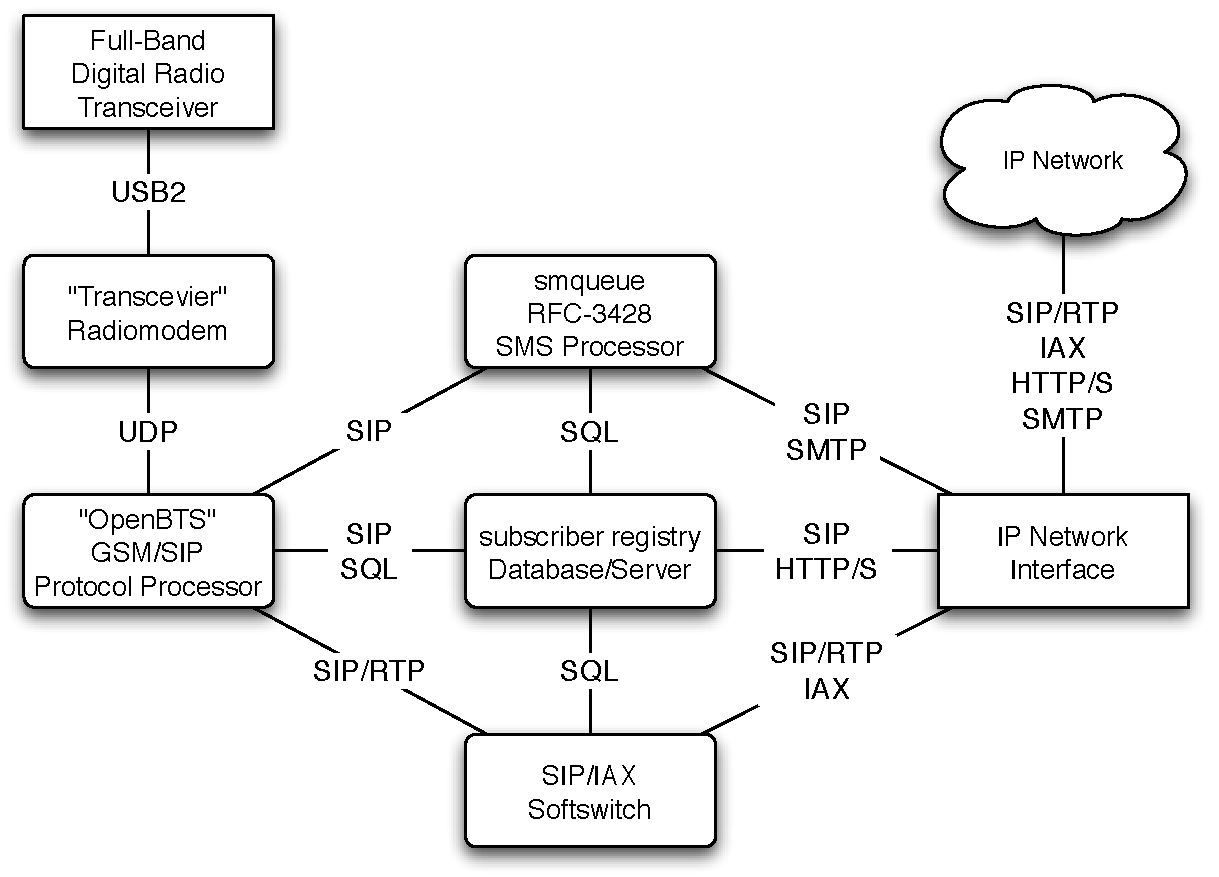
\includegraphics[width=\textwidth]{InsideTheNode.pdf}
\caption{Components of the OpenBTS application suite and their communication channels as installed in each access point.  Sharp-cornered boxes are hardware components.  Round-cornered boxes are software components.}
\label{fig:insideTheNode}
\end{center}
\end{figure}





\chapter{The OpenBTS GSM Air Interface}
\label{chap:Um}
This chapter describes the GSM air interface, ``Um'', as implemented by OpenBTS.
It is not really necessary to fully understand this chapter to use OpenBTS, but the information is given here for completeness and to provide references to important parts of the GSM specifications to support more detailed study.

Broadly speaking, Um is organized into channels and layers, as shown in Figure~\ref{fig:GSMLayers}.
The rest of this chapter will explain this diagram.

\begin{figure}[htbp]
\begin{center}
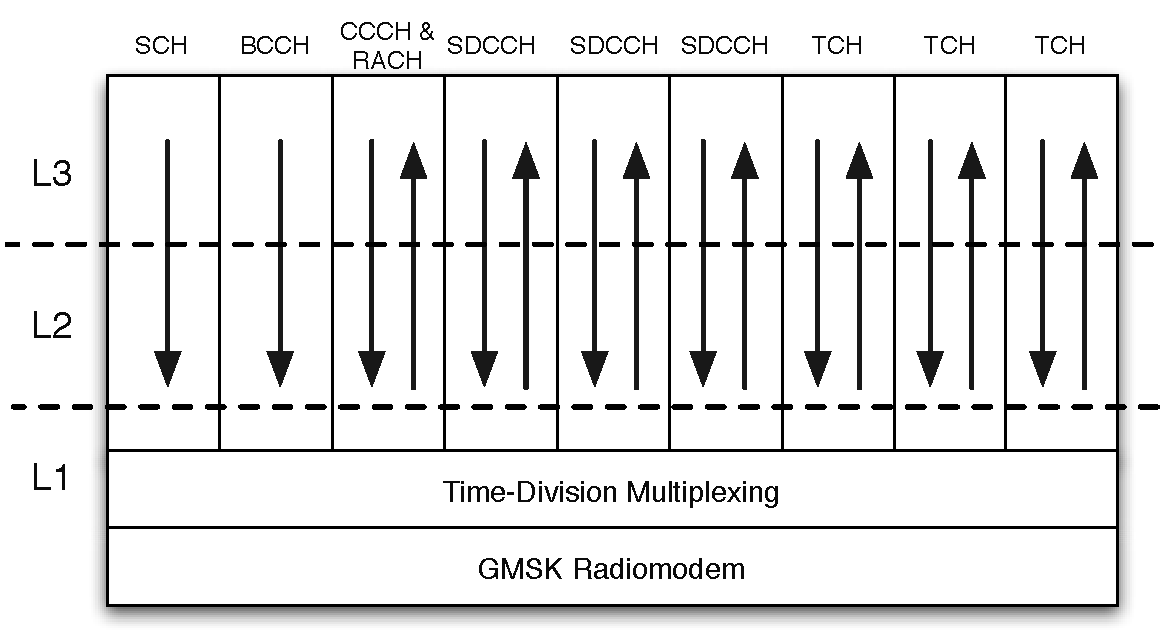
\includegraphics[width=6in]{GSMLayers.pdf}
\caption{Layers and channels of the Um interface.  This figure shows the basic logical channel types in a subset of a typical configuration.}
\label{fig:GSMLayers}
\end{center}
\end{figure}


\section{Um Layers}
The layers of GSM are initially defined in GSM~04.01 Section~7 and roughly follow the OSI model. Um is defined in the lower three layers of the model.

\subsection{Physical Layer (L1)}
The Um physical layer is defined in the GSM~05.xx series of specifications, with the introduction and overview in GSM~05.01. For most channels, Um L1 transmits and receives 184-bit control frames or 260-bit vocoder frames over the radio interface in 148-bit bursts with one burst per timeslot. There are three sublayers:
\begin{itemize}
	\item Radiomodem. This is the actual radio transceiver, defined in largely in GSM~05.04 and 05.05.
	\item Multiplexing and Timing. GSM uses TDMA to subdivide each radio channel into as many as 16 traffic channels or as many as 64 control channels. The multiplexing patterns are defined in GSM 05.02.
	\item FEC Coding. This sublayer provides bit-error concealment and recovery.  This sublayer is defined in GSM~05.03.
\end{itemize}

\subsubsection{Radiomodem}
\label{sec:radiomodem}
OpenBTS~P2.8 supports GMSK modulation with a 13/48~MHz (270.833~kHz) symbol rate and a channel spacing of 200~kHz. Since adjacent channels overlap, the standard does not allow adjacent channels to be used in the same cell. 
OpenBTS~P2.8 supports the four most common GSM bands:
\begin{itemize}
	\item GSM850, used in parts of ITU region 2
	\item PGSM900 and EGSM900, used in most of the world
	\item DCS1800, used in most of the world
	\item PCS1900, used in parts of ITU region 2
\end{itemize}

GSM is frequency duplexed, meaning that the network and MS transmit on different frequencies, allowing the BTS to transmit and receive at the same time.
Transmission from the network to the MS is called ``downlink''.
Transmission from the MS to the network is called ``uplink''.
GSM uplink and downlink bands are separated by 45 or 50~MHz, depending on the specific band.

Uplink/downlink channel pairs are identified by an index called the ARFCN. Within the BTS, these ARFCNs are given arbitrary carrier indexes C0, C1, etc., with C0 designated as a Beacon Channel and always operated at constant power.
The radio channel is time-multiplexed into 8 timeslots, each with a duration of 156.25 symbol periods. These 8 timeslots form a frame of 1,250 symbol periods. The capacity associated with a single timeslot on a single ARFCN is called a physical channel (PCH) and referred to as ``C$n$T$m$'' where $n$ is a carrier index and $m$ is a timeslot index (0-7).

Each timeslot is occupied by a radio burst with a guard interval, two payload fields, tail bits, and a midamble (or training sequence). The lengths of these fields vary with the burst type but the total burst length is always 156.25 symbol periods. The most commonly used burst is the Normal Burst (NB).
There are several other burst formats, though. Bursts that require higher processing gain for signal acquisition have longer midambles. The random access burst (RACH) has an extended guard period to allow it to be transmitted with incomplete timing acquisition. Burst formats are described in GSM 05.02 Section 5.2.

\subsubsection{Multiplexing and Timing}
Each physical channel is time-multiplexed into multiple logical channels according to the rules of GSM~05.02. Traffic channel multiplexing follows a 26-frame (0.12 second) cycle called a "multiframe". Control channels follow a 51-frame multiframe cycle.  The C0T0 physical channel carries the SCH, which encodes the timing state of the BTS to facilitate synchronization to the TDMA pattern.

GSM timing is driven by the serving BTS through the SCH and FCCH. All clocks in the MS, including the symbol clock and local oscillator, are slaved to signals received from the BTS, as described in GSM 05.10. BTSs in the GSM network can be asynchronous, so that each BTS can run an independent clock.

\subsubsection{FEC Coding}
The coding sublayer provides forward error correction. As a general rule, each GSM channel uses a block parity code (usually a Fire code), a rate-1/2, 4th-order convolutional code and a 4-burst or 8-burst interleaver. Notable exceptions are the synchronization channel (SCH) and random access channel (RACH) that use single-burst transmissions and thus have no interleavers. For speech channels, vocoder bits are sorted into importance classes with different degrees of encoding protection applied to each class (GSM 05.03).
Using soft-input Viterbi decoding, the FEC decoders in OpenBTS can recover frames reliably with bit erasure rates in excess of 25\%.

Most channels in GSM use 456-bit L1 frames. On channels with 4-burst interleaving (BCCH, CCCH, SDCCH, SACCH), these 456 bits are interleaved in to 4 radio bursts with 114 payload bits per burst. On channels with 8-burst interleaving (TCH, FACCH), these 456 bits are interleaved over 8 radio bursts so that each radio burst carries 57 bits from the current L1 frame and 57 bits from the previous L1 frame. Interleaving algorithms for the most common traffic and control channels are described in GSM~05.03 Sections 3.1.3, 3.2.3 and 4.1.4.

\subsection{Data Link Layer (L2)}
The Um data link layer, LAPDm, is defined in GSM 04.05 and 04.06. LAPDm is the mobile analog to ISDN's LAPD and like LAPD, LAPDm is a simplified form of HDLC.

\subsection{Network Layer (L3)}
Um L3 is defined in GSM~04.07 and 04.08 and has three sublayers. A subscriber terminal must establish a connection in each sublayer before accessing the next higher sublayer.
\begin{itemize}
	\item Radio Resource (RR). This sublayer manages the assignment and release of logical channels on the radio link. It is normally terminated in the BSC, although in OpenBTS, RR is terminated locally in the OpenBTS stack.
	\item Mobility Management (MM). This sublayer authenticates users and tracks their movements from cell to cell. OpenBTS translates MM transactions into corresponding SIP transactions and uses the Asterisk SIP registry to perform MM functions.
	\item Call Control (CC). This sublayer connects telephone calls and is taken directly from ITU-T~Q.931. GSM~04.08 Annex E provides a table of corresponding paragraphs in GSM~04.08 and ITU-T~Q.931 along with a summary of differences between the two. In OpenBTS, CC transactions are translated to corresponding SIP transactions and processed in Asterisk.
\end{itemize}
The access order is RR, MM, CC. The release order is the reverse of that.

\section{Um logical channels}
Um logical channel types are outlined in GSM 04.03. Broadly speaking, non-GRPS Um logical channels fall into three categories: traffic channels, dedicated control channels and non-dedicated control channels.


\subsection{Traffic channels (TCH)}
These point-to-point channels correspond to the ISDN B channel and are referred to as Bm channels. Traffic channels use 8-burst diagonal interleaving with a new block starting on every fourth burst and any given burst containing bits from two different traffic frames. This interleaving pattern makes the TCH robust against single-burst fades since the loss of a single burst destroys only 1/8 of the frame's channel bits (a 12.5\% bit erasure). The coding of a traffic channel is dependent on the traffic or vocoder type employed, with most coders capable of overcoming single-burst losses. All traffic channels use a 26-multiframe TDMA structure.

\subsubsection{Full-rate channels (TCH/F)}
A GSM full rate channel uses 24 frames out of a 26-multiframe. The channel bit rate of a full-rate GSM channel is 22.7~kbit/s, although the actual payload data rate is 9.6-14 kbit/s, depending on the channel coding. OpenBTS~P2.8 supports only the GSM full-rate codec (GSM~06.10) as a media type on this channel.

\subsection{Dedicated Control Channels (DCCHs)}
These point-to-point channels correspond to the ISDN D channel and are referred to as Dm channels.

\subsubsection{Standalone Dedicated Control Channel (SDCCH)}
The SDCCH is used for most short transactions, including initial call setup step, registration and SMS transfer. It has a payload data rate of 0.8 kbit/s. Up to eight SDCCHs can be time-multiplexed onto a single physical channel. The SDCCH uses 4-burst block interleaving in a 51-multiframe.  One SDCCH channel can be used to process 10-15 location updates per minute or to transfer 5-10 SMS per minute.

\subsubsection{Fast Associated Control Channel (FACCH)}
The FACCH is always paired with a traffic channel. The FACCH is a blank-and-burst channel that operates by stealing bursts from its associated traffic channel. Bursts that carry FACCH data are distinguished from traffic bursts by stealing bits at each end of the midamble. The FACCH is used for in-call signaling, including call disconnect, handover and the later stages of call setup. It has a payload data rate of 9.2 kbit/s when paired with a full-rate channel (FACCH/F) and 4.6 kbit/s when paired with a half-rate channel (FACCH/H). The FACCH uses the same interleaving and multiframe structure as its host TCH.

\subsubsection{Slow Associated Control Channel (SACCH)}
Every SDCCH or FACCH also has an associated SACCH. Its normal function is to carry system information messages 5 and 6 on the downlink, carry receiver measurement reports on the uplink and to perform closed-loop power and timing control. Closed loop timing and power control are performed with a physical header at the start of each L1 frame. This 16-bit physical header carries actual power and timing advance settings in the uplink and ordered power and timing values in the downlink. The SACCH can also be used for in-call delivery of SMS. The SACCH has a payload data rate of 0.2-0.4~kbit/s, depending on the channel with which it is associated. The SACCH uses 4-burst block interleaving and the same multiframe type as its host TCH or SDCCH.

\subsection{Non-Dedicated Control Channels (NDCCHs)}
These are unicast and broadcast channels that do not have analogs in ISDN. These channels are used almost exclusively for radio resource management. The CCCH and RACH together form the medium access mechanism for Um.

\subsubsection{Broadcast Control Channel (BCCH)}
The BCCH carries a repeating pattern of system information messages that describe the identity, configuration and available features of the BTS. BCCH brings the measurement reports it bring the information about LAI And CGI BCCH frequency are fixed in BTS.
The C0T0 beacon channel must carry an instance of the BCCH.

\subsubsection{Synchronization Channel (SCH)}
The SCH transmits a Base station identity code and the current value of the TDMA clock.
The C0T0 beacon channel must carry an instance of the SCH.

\subsubsection{Frequency Correction Channel (FCCH)}
The FCCH generates a tone on the radio channel that is used by the MS to discipline its local oscillator.

\subsubsection{Common Control Channel (CCCH)}
The CCCH is a downlink unicast channel that carries paging requests and channel assignment messages (specifically, immediate assignment messages). The CCCH is subdivided into the paging channel (PCH) and access grant channel (AGCH). An MS that is camped to a BTS monitors the PCH for service notifications from the network.

\subsubsection{Random Access Channel (RACH)}
The RACH is the uplink counterpart to the CCCH. The RACH is a shared channel on which the MSs transmit random access bursts to request channel assignments from the BTS, assignments which are granted on the AGCH part of the CCCH.

\subsection{Allowed channel combinations}
The multiplexing rules of GSM 05.02 allow only certain combinations of logical channels to share a physical channel. The combinations supported by OpenBTS~P2.8 are:
\begin{itemize}
	\item Combination I: TCH/F + FACCH/F + SACCH. This combination is used for full rate traffic. It can be used anywhere but C0T0.
	\item Combination V: FCCH + SCH + BCCH + CCCH + 4 SDCCH + 4 SACCH. This is the typical C0T0 beacon channel combination for small cells. It can be used only on C0T0.  Since this is the only beacon channel combination supported by OpenBTS P2.8, it \emph{must} be used on C0T0.
	\item Combination VII: 8 SDCCH + 8 SACCH. This combination is used to provide additional SDCCH capacity in situations where registration loads or SMS usage may be particularly heavy. It can be used anywhere but C0T0.
\end{itemize}





\section{Service Capacity of Um}
The capacities of OpenBTS products, ARFCN-for-ARFCN, are the same as for any other GSM basesations. The only exception to this is that OepnBTS P2.8 doe not support half-rate channels.

OpenBTS P2.8 offers two types of dedicated channels:
\begin{itemize}
	\item Full-Rate Traffic Channel (TCH/F).  Each Combination-I slot contains a single TCH/F that can carry a single speech call.
	\item Standalone Dedicated Control Channel (SDCCH).  Each Combination-VII slot carries eight SDCCHs.  The Combination-V beacon also carries four SDCCHs.  Each SDCCH can process about 30 authenticated registration transactions per minute or transfer about 12 text messages per minute, assuming good link margins.  \emph{Bear in mind that poor link margins will significantly degrade SDCCH capacity by forcing retransmission of L2 frames and requiring long tear-down times for dropped channels.}
\end{itemize}

A typical configuration for a single-ARFCN BTS in a speech-oriented application is
\begin{itemize}
	\item a Combination-IV beacon on C0T0 carrying 4 SDCCHs and
	\item six Combination-I slots on C0T1-C0T7 carrying  total of 7 TCH/Fs.
\end{itemize}
This combination would typically support about about 15 authenticated registrations per minute, about 40 text messages per minute and seven concurrent calls.  The number of subscribers that can actually be served with that capacity will be covered in the following sections.










\chapter{External Databases}
\label{chap:databases}
OpenBTS~P2.8 uses a set of sqlite3 database files to make its configuration and status information available to external applications.
Sqlite3 is a self-contained, serverless SQL database, originally developed for guided missile systems and now used many well-known applications, including the Blackberry, Symbian, iOS and Android operating systems.  For more information on sqlite3, see the www.sqlite.org web site.

\section{Editing Sqlite3 Databases}
\label{sec:sqlite3Tools}
The following methods can be used to edit or view the OpenBTS sqlite3 database files:
\begin{itemize}
	\item The sqlite3 command line tool. Range Networks access points include the sqlite3 command line tool that can be used to inspect and modify these databases using SQL syntax.
	\begin{itemize}
		\item The database can be manipulated directly using SQL syntax in real time.
		\item For offline editing, sqlite3 can export SQL code to a text file with ``.dump''.  The text can then be edited and reimported with ``.read''.
	\end{itemize}
	\item Third-party database editors.  Generic GUI-based editors are available for sqlite3 database files.  Examples:
	\begin{itemize}
		\item ``SQLite Database Browser'' -- A free browser for OS X and Linux available from sourceforge.net.
		\item ``RazorSQL'' -- A commercial database GUI available from razorsql.com.
		\item Firefox -- Mozilla offers a free Firefox add-on called SQLite Manager that allows the Firefox web browser to be used to view and edit sqlite3 databases, available from addons.mozilla.org.
	\end{itemize}
	\item OpenBTS itself.  The OpenBTS CLI ``config'' and ``unconfig'' commands (Section~\ref{sec:CLI}) can be used to edit the configuration table (Section~\ref{sec:configTable}) in real time.  Configuration changes from the CLI are written back the to OpenBTS.db database and are persistent.

\end{itemize}

\section{The Configuration Table}
\label{sec:configTable}
The parameters that control the OpenBTS application are stored in a database table called the \emph{configuration table}.  Some parameters are \emph{dynamic}, meaning that a parameter change will have an immediate effec.  Some of these parameters are \emph{static} and changes to them do not take effect until OpenBTS is restarted.  Some of these static parameters are matched to the hardware of a specific implementation and should not be changed at all.  Comments within the configuration database describe each parameter and under what conditions it can be changed.
Flags within the database schema indicate which parameters are static.
The schema for the P2.8 configuration table is:
\begin{verbatim}
CREATE TABLE CONFIG (
    KEYSTRING TEXT UNIQUE NOT NULL, 
    VALUESTRING TEXT, 
    STATIC INTEGER DEFAULT 0, 
    OPTIONAL INTEGER DEFAULT 0, 
    COMMENTS TEXT DEFAULT ''
)
\end{verbatim}

Note that the database itself contains comments, available to the operator at all times and repeated in this manual.

To change a dynamic configuration parameter in real time, edit the table using one of the methods described in Section~\ref{sec:sqlite3Tools}.  The effect will be immediate, although in-progress transactions may continue to use the parameters with which they started.  (For example, a change in SIP.Proxy.Speech will not affect in-progress telephone calls, but any new calls will use the new proxy.)

To change a static configuration parameter. edit the table using one of the methods described in Section~\ref{sec:sqlite3Tools} and then restart the OpenBTS application.
In standard-configuration embedded Linux systems, this restart can be accomplished with the ``exit'' command, described in Section~\ref{sec:exitCmd} or by rebooting the BTS unit.

In some cases, NULL is a valid value for a configuration parameter.  In SQL terminology, the NULL value is a special tag that indicates that a value is not defined.  This is not the same as the string ``NULL'', which is an actual string value with a value of ``NULL''.  To make a value NULL from the CLI, use the ``unconfig'' command.

The configuration parameters are listed here briefly, but some parameters of particular importance are covered in later sections.


\begin{itemize}
\item CLI.Prompt -- Prompt for the OpenBTS command line interface.
\item Control.Emergency.Destination.Host -- SIP destination host to be used for the "To:" header of emergency calls.  This host may be different from the address given for SIP.Proxy.Emergency.
\item Control.Emergency.Destination.User -- SIP destination user or extension to be used for the "To:" header of emegency calls.  IMS specifies "sos", but correct value must be matched to your switch configuration and PSAP interface.
\item Control.Emergency.GatewaySwitch -- Gateway SIP switch for inbound calls from other networks.  This host is used to form the return path for emergency calls, so it should be a host address that will route from your serving PSAP.
\item Control.Emergency.Geolocation -- If defined, send this location as an RFC-4119 XML GEOPRIV object during SIP emergency call establishment.  Format is dd:mm:ss[NS] ddd:dd:dd[EW].
\item Control.Emergency.QueueTime -- Maximum time to wait for a channel to open up for an emegency call in a congested system, in milliseconds.
\item Control.Emergency.RFC5031 -- If not NULL, use the RFC-5031 URN sip:sos@SIP.Proxy.Emergency as the request URN for outbound emergency calls over SIP, regardless of the value of Emergency.Destination.User.  The "To:" header will still be Emergency.Destination.User@Emergency.Destination.Host.
\item Control.Emergency.Source.User -- SIP identity to use if no IMSI is available.  IMS specifies "anonymous" but other values might be more useful depending on your configuration.
\item Control.GSMTAP.TargetIP -- Target IP address for GSMTAP packets; the IP address of Wireshark, if you use it for GSM.
\item Control.LUR.AttachDetach -- Attach/detach flag.  Set to 1 to use attach/detach procedure, 0 otherwise.  This will make initial LUR more prompt.  It will also cause an un-regstration if the handset powers off and really heavy LUR loads in areas with spotty coverage.
\item Control.LUR.CachedAuthentication -- If not NULL, use RAND-SRES pairs cached in the TMSI table for authentication.  If this method is used, it is important that the TMSI Table be in persistent storage.
\item Control.LUR.DefaultAuthenticationAccept -- If not NULL, provisioned handsets will be accepted for authentication in the absence of any defined authentication method.  For commercial networks this value should probably be NULL.
\item Control.LUR.FailedRegistration.Message -- If defined, send this text message, followed by the IMSI, to unprovisioned handsets that are denied  registration.
\item Control.LUR.FailedRegistration.ShortCode -- The return address for the failed registration message.  If the message is defined, this must also be defined.
\item Control.LUR.NormalRegistration.Message -- If defined, send this text message, followed by the IMSI, to provisioned handsets when they attach on Um.
\item Control.LUR.NormalRegistration.ShortCode -- The return address for the normal registration message.  If the message is defined, this must also be defined.
\item Control.LUR.OpenRegistration -- A regular expression.  If not NULL, allow unprovisioned handsets with matching IMSIs to attach in Um.
\item Control.LUR.OpenRegistration.Message -- If defined, send this text message, followed by the IMSI, to unprovisioned handsets when they attach on Um due to open registration.
\item Control.LUR.OpenRegistration.ShortCode -- The return address for the open registration message.  If the message is defined, this must also be defined.
\item Control.LUR.QueryClassmark -- If not NULL, query every MS for classmark during LUR.
\item Control.LUR.QueryIMEI -- If not NULL, query every MS for IMSI during LUR.
\item Control.LUR.SR-HTTPAuthentication -- If not NULL, use the HTTP interface of the subscriber registry server for authentication.
\item Control.LUR.SendTMSIs -- If not NULL, send new TMSI assignments to handsets that are allowed to attach.
\item Control.LUR.UnprovisionedRejectCause -- Reject cause for location updating failures for unprovisioned phones.  Reject causes come from GSM 04.08 10.5.3.6.  Reject cause 0x04, IMSI not in VLR, is usually the right one.
\item Control.NumSQLTries -- Number of times to retry SQL queries before declaring a database access failure.
\item Control.Reporting.PhysStatusTable -- File path for channel status reporting database.  Static.
\item Control.Reporting.TMSITable -- File path for TMSITable database.  Static.
\item Control.TMSITable.MaxAge -- Maximum allowed age for a TMSI in hours.
\item Control.TMSITable.MaxSize -- Maximum size of TMSI table before oldest TMSIs are discarded.
\item Control.TestCall.Port -- Port for exchanging L3 packets with the testcall feature.
\item Control.VEA -- If not NULL, user very early assignment for speech call establishment.  See GSM 04.08 Section 7.3.2 for a detailed explanation of assignment types. If VEA is selection, GSM.CellSelection.NECI should be set to 1.  See GSM 04.08 Sections 9.1.8 and 10.5.2.4 for an explanation of the NECI bit.
\item GSM.CCCH.AGCH.QMax -- Maximum number of access grants to be queued for transmission on AGCH before declaring congrestion.
\item GSM.CCCH.CCCH-CONF -- CCCH configuration type.  See GSM 10.5.2.11 for encoding.  Value of 1 means we are using a C-V beacon.  Any other value selects a C-IV beacon.
\item GSM.CCCH.PCH.Reserve -- Number of CCCH subchannels to reserve for paging.
\item GSM.CellSelection.CELL-RESELECT-HYSTERESIS -- Cell Reselection Hysteresis.  See GSM 04.08 10.5.2.4, Table 10.5.23 for encoding.  Encoding is $2N$ dB, values of $N$ are 0...7 for 0...14 dB.
\item GSM.CellSelection.MS-TXPWR-MAX-CCH -- Cell selection parameters.  See GSM 04.08 10.5.2.4.
\item GSM.CellSelection.NCCsPermitted -- NCCs Permitted.  An 8-bit mask of allowed NCCs.  Unless you are coordinating with another carrier, this should probably just select your own NCC.
\item GSM.CellSelection.NECI -- NECI, New Establishment Causes.  This must be set to "1" if you want to support very early assignment.  See GSM 04.08 10.5.2.4, Table 10.5.23 and 04.08 9.1.8, Table 9.9.
\item GSM.CellSelection.Neighbors -- ARFCNs of neighboring cells.
\item GSM.CellSelection.RXLEV-ACCESS-MIN -- Cell selection parameters.  See GSM 04.08 10.5.2.4.
\item GSM.Channels.C1sFirst -- If not NULL, allocate C-I slots first, starting at C0T1.  Otherwise, allocate C-VII slots first.  Static.
\item GSM.Channels.NumC1s -- Number of Combination-I timeslots to configure.  The C-I slot carries a single full-rate TCH, used for speech calling.  Static.
\item GSM.Channels.NumC7s -- Number of Combination-VII timeslots to configure.  The C-VII slot carries 8 SDCCHs, useful to handle high registration loads or SMS.  If C0T0 is C-IV, you must have at least one C-VII also.  Static.
\item GSM.Identity.BSIC.BCC -- GSM basestation color code; lower 3 bits of the BSIC.  BCC values in a multi-BTS network should be assigned so that BTS units with overlapping coverage do not share a BCC.  This value will also select the training sequence used for all slots on this unit.
\item GSM.Identity.BSIC.NCC -- GSM network color code; upper 3 bits of the BSIC.  Assigned by your national regulator.  Must be distinct from NCCs of other GSM operators in your area.
\item GSM.Identity.CI -- Cell ID, 16 bits.  Should be unique.
\item GSM.Identity.LAC -- Location area code, 16 bits, values 0xFFxx are reserved.  For multi-BTS networks, assign a unique LAC to each BTS unit.  (That is not the normal procedure in conventional GSM networks, but is the correct procedure in OpenBTS networks.)
\item GSM.Identity.MCC -- Mobile country code, 2 or 3 digits.  Defined in ITU-T E.212.
\item GSM.Identity.MNC -- Mobile network code; Must be 3 dgits.  Assigned by your national regulator.
\item GSM.Identity.ShortName -- Network short name, displayed on some phones.  Optional but must be defined if you also want the network to send time-of-day.
\item GSM.Identity.ShowCountry -- If not NULL, tell the phone to show the country name based on the MCC.
\item GSM.MS.Power.Damping -- Damping value for MS power control loop.
\item GSM.MS.Power.Max -- Maximum commanded MS power level in dBm.
\item GSM.MS.Power.Min -- Minimum commanded MS power level in dBm.
\item GSM.MS.TA.Damping -- Damping value for timing advance control loop.
\item GSM.MS.TA.Max -- Maximum allowed timing advance in symbol periods.  Ignore RACH bursts with delays greater than this.  Can be used to limit service range.
\item GSM.MaxSpeechLatency -- Maximum allowed speech buffering latency, in 20 ms frames.  If the jitter is larger than this delay, frames will be lost.
\item GSM.RACH.AC -- Access class flags.  This is the raw parameter sent on the BCCH.  See GSM 04.08 10.5.2.29 for encoding.  Set to 0 to allow full access.  If you do not have proper PSAP integration, set to 0x0400 to indicate no support for emergency calls.
\item GSM.RACH.MaxRetrans -- Maximum RACH retransmission attempts.  This is the raw parameter sent on the BCCH.  See GSM 04.08 10.5.2.29 for encoding.
\item GSM.RACH.TxInteger -- Parameter to spread RACH busts over time.  This is the raw parameter sent on the BCCH.  See GSM 04.08 10.5.2.29 for encoding.
\item GSM.RADIO-LINK-TIMEOUT --  L1 radio link timeout.  This is the raw parameter sent on the BCCH; see GSM 10.5.2.3 for encoding. Should be coordinated with T3109.
\item GSM.RRLP.ACCURACY -- Requested accuracy of location request. K in 10(1.1**K-1). See 3GPP 03.32, sect 6.2
\item GSM.RRLP.ALMANAC.REFRESH.TIME -- How often the almanac is refreshed, in hours
\item GSM.RRLP.ALMANAC.URL -- URL of almanac source.
\item GSM.RRLP.EPHEMERIS.REFRESH.TIME -- How often the ephemeris is refreshed, in hours.
\item GSM.RRLP.EPHEMERIS.URL -- URL of ephemeris source.
\item GSM.RRLP.RESPONSETIME -- Mobile timeout. (OpenBTS timeout is 130 sec = max response time + 2.) N in 2**N. See 3GPP 04.31 sect A.2.2.1
\item GSM.RRLP.SEED.ALTITUDE -- Seed altitude in meters wrt geoidal surface.
\item GSM.RRLP.SEED.LATITUDE -- Seed latitude in degrees.  -90 (south pole) .. +90 (north pole)
\item GSM.RRLP.SEED.LONGITUDE -- Seed longitude in degrees.  -180 (west of greenwich) .. 180 (east)
\item GSM.RRLP.SERVER.URL -- URL of RRLP server.
\item GSM.Radio.Band -- The GSM operating band.  Valid values are 850 (GSM850), 900 (PGSM900), 1800 (DCS1800) and 1900 (PCS1900).  For most Range models, this value is dictated by the hardware and should not be changed.  Static.
\item GSM.Radio.C0 -- The C0 ARFCN. Static.
\item GSM.Radio.MaxExpectedDelaySpread -- Expected worst-case delay spread in symbol periods, roughly 3.7 us or 1.1 km per unit.
\item GSM.Radio.PowerManager.MaxAttenDB -- Maximum transmitter attenuation level, in dB wrt full scale on the D/A output.  This sets the minimum power output level in the output power control loop.
\item GSM.Radio.PowerManager.MinAttenDB -- Minimum transmitter attenuation level, in dB wrt full scale on the D/A output.  This sets the maximum power output level in the output power control loop.
\item GSM.Radio.PowerManager.NumSamples -- Number of samples averaged by the output power control loop.
\item GSM.Radio.PowerManager.SamplePeriod -- Sample period for the output power control loop.
\item GSM.Radio.PowerManager.TargetT3122 -- Target value for T3122, the random access hold-off timer, for the power control loop.
\item GSM.Radio.RSSITarget -- Target uplink RSSI for MS power control loop, in dB wrt to A/D full scale.  Should be 6-10 dB above the noise floor.
\item GSM.Radio.RxGain -- Receiver gain setting in dB.  Ideal value is dictacted by the hardware.  This database parameter is static but the receiver gain can be modified in real time with the CLI rxgain command.  Static.
\item GSM.Timer.T3113 -- Paging timer T3113 in ms.  This is the timeout for a handset to respond to a paging request.  This should usually be the same as SIP.Timer.B in your VoIP network.
\item GSM.Timer.T3122Max -- Maximum allowed value for T3122, the RACH holdoff timer, in milliseconds.
\item GSM.Timer.T3122Min -- Minimum allowed value for T3122, the RACH holdoff timer, in milliseconds.
\item GSM.Timer.T3212 -- Registration timer T3212 period in minutes.  Should be a factor of 6.  Set to 0 to disable periodic registration.  Should be smaller than SIP registration period.
\item Log.Alarms.Max -- Maximum number of alarms to remember inside the application.
\item Log.Level -- Default logging level when no other level is defined for a file.
\item Log.Level.CallControl.cpp -- Default configuration logs a trace at L3.
\item Log.Level.MobilityManagement.cpp -- Default configuration logs a trace at L3.
\item Log.Level.RadioResource.cpp -- Default configuration logs a trace at L3.
\item Log.Level.SMSControl.cpp -- Default configuration logs a trace at L3.
\item NTP.Server -- NTP server(s) for time-of-day clock syncing.  For multiple servers, use a space-delimited list.  If left undefined, NTP will not be used, but it is strongly recommended.
\item RTP.Range -- Range of RTP port pool.  Pool is RTP.Start to RTP.Range-1.  Static.
\item RTP.Start -- Base of RTP port pool.  Pool is RTP.Start to RTP.Range-1.  Static.
\item SIP.DTMF.RFC2833 -- If not NULL, use RFC-2833 (RTP event signalling) for in-call DTMF.
\item SIP.DTMF.RFC2833.PayloadType -- Payload type to use for RFC-2833 telephone event packets.  If SIP.DTMF.2833 is defined, this must also be defined.
\item SIP.DTMF.RFC2967 -- If not NULL, use RFC-2967 (SIP INFO method) for in-call DTMF.
\item SIP.Local.IP -- IP address of the OpenBTS machine as seen by its proxies.  If these are all local, this can be localhost.  Static.
\item SIP.Local.Port -- IP port that OpenBTS uses for its SIP interface.  Static.
\item SIP.MaxForwards -- Maximum allowed number of referrals.
\item SIP.Proxy.Emergency -- The IP host and port of the proxy to be used for emergency calls.
\item SIP.Proxy.Registration -- The IP host and port of the proxy to be used for registration and authentication.  This is the subscriber registry, for example.
\item SIP.Proxy.SMS -- The IP host and port of the proxy to be used for text messaging.  This is smqueue, for example.
\item SIP.Proxy.Speech -- The IP host and port of the proxy to be used for normal speech calls.  This is Asterisk, for example.
\item SIP.RegistrationPeriod -- Registration period in minutes for MS SIP users.  Should be longer than GSM T3212.
\item SIP.SMSC -- The SMSC handler in smqueue.  This is the entity that handles full 3GPP MIME-encapsulted TPDUs.  If not defined, use direct numeric addressing.  Normally the value is NULL if SMS.MIMIEType is "text/plain" or "smsc" if SMS.MIMEType is "application/vnd.3gpp".
\item SIP.Timer.A -- INVITE retransmit period in ms.
\item SIP.Timer.B -- INVITE transaction timeout in ms.  This value should usually match GSM.Timer.T3113.
\item SIP.Timer.E -- Non-INVITE initial request retransmit period in ms.
\item SIP.Timer.F -- Non-INVITE initial request timeout in ms.
\item SIP.Timer.H -- ACK timeout period in ms.
\item SIP.Timer.I -- ACK retransmit period in ms.
\item SIP.Timer.J -- Non-INVITE non-initial request retransmit period in ms.
\item SIP.myPort -- Port used by the SIP Authentication Server
\item SMS.DefaultDestSMSC -- Use this to fill in L4 SMSC address in SMS submission.
\item SMS.FakeSrcSMSC -- Use this to fill in L4 SMSC address in SMS delivery.
\item SMS.MIMEType -- This is the MIME Type that OpenBTS will use for RFC-3428 SIP MESSAGE payloads.  Valid values are "application/vnd.3gpp.sms" and "text/plain".
\item SubscriberRegistry.A3A8 -- URL of upstream subscriber registry server.  Blank (not NULL) if there is none.
\item SubscriberRegistry.HTTP.Server -- URL of the subscriber registry server.
\item SubscriberRegistry.Manager.Title -- Title of subscriber registry database manager web page.
\item SubscriberRegistry.Manager.Url -- URL of the subscriber registry database manager.
\item SubscriberRegistry.Manager.VisibleColumns -- Field names in subscriber registry visible in the database manager.
\item SubscriberRegistry.db -- The location of the sqlite3 database holding the subscriber registry.
\item TRX.IP -- IP address of the transceiver application.  Static.
\item TRX.Port -- IP port of the transceiver application.  Static.
\item TRX.RadioFrequencyOffset -- Fine-tuning adjustment for the transceiver.  Static.
\end{itemize}



\section{TMSI Table}
\label{sec:TMSITable}
To reduce dependence on a backhaul link, OpenBTS tracks TMSIs internally.
To accomplish this, OpenBTS tracks TMSI-IMSI relationships in an sqlite3 database table called the \emph{TMSI table}.
TMSIs are assigned by a counter in increasing order.
OpenBTS allocates a TMSI in the TMSI table for \emph{every} MS that sends a Location Updating Request, whether the MS is allowed to register or not.

The TMSI table is treated as read-write by OpenBTS but should be treated as read-only by other applications.
The path of the database file used for this table is defined in the configuration parameter Control.DBPath.TMSITable.  In flash-based systems, this table should be stored in a ramdisk partition and its standard location is in /var/run.  The schema is:
\begin{verbatim}
CREATE TABLE IF NOT EXISTS TMSI_TABLE (
  TMSI INTEGER PRIMARY KEY AUTOINCREMENT -- this value is used as the TMSI
  CREATED INTEGER NOT NULL, -- Unix time of record creation
  ACCESSED INTEGER NOT NULL,  -- Unix time of last encounter
  IMSI TEXT UNIQUE NOT NULL, -- IMSI of the SIM
  IMEI TEXT, -- IMEI of the MS, if requested
  L3TI INTEGER DEFAULT 0, -- L3 transaction identifier last used with this MS
  A5_SUPPORT INTEGER, -- encryption support in the MS, if requested
  POWER_CLASS INTEGER,  -- power class of the MS. if requested
  OLD_TMSI INTEGER,  -- previous TMSI from another cell or network
  PREV_MCC INTEGER, -- previous network MCC
  PREV_MNC INTEGER,  -- previous network MNC
  PREV_LAC INTEGER, -- previous network LAC
  RANDUPPER INTEGER -- cached authentication token
  RANDLOWER INTEGER -- cached authentication token
  SRES INTEGER, -- cached authentication token
  DEG_LAT FLOAT, -- cached RRLP result
  DEG_LONG FLOAT -- cached RRLP result
)
\end{verbatim}




\section{Channel Table}
\label{sec:channelTable}
OpenBTS reports real-time physical status information for active dedicated channels to an external sqlite3 database table called PHYSTATUS.
This table is treated as write-only by OpenBTS but should be treated as read-only by other applications.  The entry for a channel is updated every time a system information message is received on the channel's associated SACCH.
The path of the database file used for this table is defined in the configuration parameter GSM.DBPath.PhysStatusTable.  The schema is:

% TODO: This needs to be updated.
\begin{verbatim}
CREATE TABLE IF NOT EXISTS PHYSTATUS (
  CN_TN_TYPE_AND_OFFSET STRING PRIMARY KEY,  -- cross-refs TRANSACTION_TABLE
  ARFCN INTEGER DEFAULT NULL, -- actual ARFCN
  ACCESSED INTEGER DEFAULT 0,  -- Unix time of last update
  RXLEV_FULL_SERVING_CELL INTEGER DEFAULT NULL,  -- from most recent measurement report
  RXLEV_SUB_SERVING_CELL INTEGER DEFAULT NULL,   -- from most recent measurement report
  RXQUAL_FULL_SERVING_CELL_BER FLOAT DEFAULT NULL, -- from most recent measurement report
  RXQUAL_SUB_SERVING_CELL_BER FLOAT DEFAULT NULL, -- from most recent measurement report
  RSSI FLOAT DEFAULT NULL, -- RSSI relative to full scale input
  TIME_ERR FLOAT DEFAULT NULL,  -- timing advance error in symbol periods
  TRANS_PWR INTEGER DEFAULT NULL, -- MS tx power in dBm
  TIME_ADVC INTEGER DEFAULT NULL, -- MS timing advance in symbol periods
  FER FLOAT DEFAULT NULL -- uplink FER
)
\end{verbatim}

The CN\_TN\_TYPE\_AND\_OFFSET field is a channel description string of the form
\begin{verbatim}
C<n>T<n> <channelType>-<subchannelIndex>
\end{verbatim}
For example
\begin{itemize}
	\item ``C0T1 TCH/F'' is a full rate traffic channel on timeslot 1 of the C0 ARFCN and 
	\item ``C0T0 SDCCH-0/4'' is the \#0 SDCCH (of 4 available) on C0T0.
\end{itemize}
Strings of the same format are used in the transaction table.

 

\chapter{Processes Inside OpenBTS}
\label{chap:inside}
Along with the fundamental channels and layers described in Chapter~\ref{chap:Um}, OpenBTS~P2.8 contains several processes that support its operation and tie the channels together to form a unified BTS.%
\footnote{The term ``process'' here does not refer to an operating system process.  Here, a ``process'' is simple an on-going activity inside the OpenBTS software.}


\section{T3122 Exponential Back-Off}
\label{sec:T3122}
When too many MSs make simultaneous access attempts to the BTS, resulting in channel exhaustion, the BTS can respond on the CCCH with an Immediate Assignment Reject message, as defined in GSM 04.08 Section 9.1.20.
This message carries a value, T3122, that dictates how long the rejected MS must wait before making another access attempt. (Emergency call attempts are not subject to T3122 waiting.)

OpenBTS implements an exponential back-off algorithm that causes T3122 to grow exponentially whenever channel exhaustion occurs.  The bounds for T3122 are set with the configuration parameters GSM.Timer.T3122Max and GSM.Timer.T3122Min, given in milliseconds. To disable the exponential back-off, set these two bounds to the same value.

T3122 back-off is connected to downlink power adaptation, described in Section~\ref{sec:powerManager}.


\section{Downlink Power and Congestion Management}
\label{sec:powerManager}
OpenBTS can automatically adjust its downlink power to limit loads and prevent congestion.  This feature is especially useful for graceful power-up in areas with very high subscriber density and load-shedding in the event of sudden failure of a neighboring cell or even the failure of a nearby cell of a different operator.  This congestion management feature works in conjunction with the T3122 adaptation loop described in Section~\ref{sec:T3122}.
The practical result of the automatic power adjustment is to limit the service area of the BTS to a population of nearby phones that it can actually serve.

The configuration parameters associated with this mechanism are:
\begin{itemize}
	\item GSM.PowerManager.TargetT3122 -- This is the acceptable value of T3122 that the power management loop attempts to achieve.  If the actual value of T3122 is larger than this, the BTS will reduce its output power.  If the actual value of T3122 is small than this, the BTS will increase its output power (if it is not already maximized).  It is critical that this target value be within the bounds set by GSM.Timer.T3122Max and GSM.Timer.T3122Min, as described in Section~\ref{sec:T3122}.
	\item GSM.PowerManager.Period -- This is the adaptation time constant in milliseconds.
	\item GSM.PowerManger.MaxAttenDB -- The maximum allowed attenuation, in dB relative to full power, which determines the minimum output level.  This is also the initial attenuation level. 
	\item GSM.PowerManager.MinAttenDB -- The minimum allowed attenuation, in dB relative to full scale, which determines the maximum output level.  This value is normally zero, allowing the BTS to operate at the maximum power level supported by the hardware.
\end{itemize}

To disable the automatic power control feature, set the minimum and maximum attenuation levels (MaxAttenDB and MinAttenDB) to the same value, usually zero for maximum power at all times.
The CLI ``power'' command, described in Section~\ref{sec:powerCmd}, can be used monitor this mechanism or to control upper and lower power bounds as a pair.


\section{Uplink Power and Timing Control}
\label{sec:closedLoop}
\subsection{Uplink Power Control}
GSM uses a closed-loop uplink power control, described in GSM 05.08 Sections 4.1-4.2 and GSM 05.05 Section 4.1.1.   The available maximum power levels of GSM MSs are given in Table~\ref{tab:MSPower}.  A multi-band MS can (and typically will) have different power classes in each supported band.
The lowest available power output in any band is 5~dBm.
The power control range is set with the configuration parameters GSM.MS.Power.Max and GSM.MS.Power.Min, both expressed in dBm. These are normally set to 5 and 39, respectively. These are global settings, applied to all MSs equally.
For example, the effect of setting GSM.MS.Power.Max to something less than 39 in a GSM900 unit is to remove any range advantage that might be had by MSs power class 2.  If an MS receives a power command that falls outside of its available power range, that MS will set its output power to the closest level available, maximum or minimum.  So there is no risk in setting these bounds wider than what the MS can actually support.
It may be desirable, though, in some installations, to limit MS power to prevent interference to other cell sites in the area.

\begin{table}[htdp]
\caption{Maximum output power levels for GSM MSs.  From GSM 05.05 Section 4.1.1.}
\begin{center}
\begin{tabular}{|c|c|c|c|}
\hline
{\bf Power} 	& {\bf GSM850 GSM900} 	& {\bf DCS1800} 	& {\bf PCS1900} \\ 
{\bf Class}		& {\bf Max.\ Ouput} 		& {\bf Max.\ Output} 	& {\bf Max.\ Output} \\ \hline \hline
1 			& N/A 				& 1 W (30 dBm) 	& 1 W (30 dBm)  \\ \hline
2 & 8 W (39 dBm) & 0.25 W (24 dBm) & 0.25 W (30 dBm) \\ \hline
3 & 5 W (33 dBm) & 4 W (36 dBm) & 2 W (33 dBm) \\ \hline
4 & 2 W (33 dBm) & N/A & N/A \\ \hline
5  & 0.8 W (29 dBm) & N/A & N/A \\ \hline
\end{tabular}
\end{center}
\label{tab:MSPower}
\end{table}%

\subsection{Uplink Timing Control}
GSM uses closed-loop timing advance control, described in GSM 05.10 Section 6.
The configuration parameter GSM.MS.TA.Max sets a limit on MS timing advance and can be used to deliberately limit the range of service. The value is expressed in symbol periods of round-trip delay, at about 550 meters per step. The normal value of this parameter is 63, which is also the maximum allowed value and corresponds to a maximum range of 35~km.


\section{Logging}
\label{sec:Logging}
OpenBTS~P2.8 logs to syslogd as facility local7.
OpenBTS defines the syslogd logging levels to mean the following:
\begin{itemize}
	\item EMERGENCY -- serious fault associated with service failure or hardware damage
	\item ALERT -- likely service disruption caused by misconfiguration, poor connectivity or some other problem not internal to the software
	\item CRITICAL -- anomalous event that is likely to degrade service
	\item ERROR -- an internal error of the software that may result in degradation of service in unusual circumstances
	\item WARNING -- an anomalous event that may indicate a degradation of normal service
	\item NOTICE -- anomalous event that probably does not affect service but may be of interest to network operators
	\item INFO -- a normal event
	\item DEBUG -- detailed information about internal data structures
\end{itemize}

Syslogd offers a range of powerful archival, reporting and notification mechanisms, including e-mail notifications and remote logging.  The reader is referred to syslogd documentation for further information on the features and configuration of that system.

The overall logging level for OpenBTS is set in the configuration variable Log.Level.  Logging levels can be set for a individual source file by defining a new configuration variable of the form ``Log.Level.\emph{filename}'' with a value equal to the desired logging level.  For example, ``Log.Level.CallControl.cpp INFO'' sets the logging level to INFO for all functions in the file CallControl.cpp.  These log levels are dynamic and can also be set and changed in real time with the ``config'' command (Section~\ref{sec:configCmd}).

Some useful logging settings are:
\begin{itemize}
	\item config Log.Level GSML2LAPDm.cpp INFO -- for an L2 trace
	\item config Log.Level RadioResource.cpp INFO -- for an L3 RR trace
	\item config Log.Level MobilityManagement.cpp INFO -- for an L3 MM trace
	\item config Log.Level CallControl.cpp INFO -- for an L3 CC trace
	\item config Log.Level.SIPInterface.cpp INFO -- for a trace of all SIP messages
	\item config Log.Level.SIPEngine.cpp INFO -- for a trace of SIP state machine activity
	\item config Log.Level.SMSControl.cpp INFO -- for a trace of L3 SMS activity
\end{itemize}

The logging destination is controlled by the configuration of syslogd or rsyslogd, depending on the host system's Unix installation.  In most configurations used by Range Networks, the logging mechanism is rsyslogd, configured with /etc/rsyslog.d/OpenBTS.conf.  The standard configuration is:
\begin{verbatim}
local7.*                        /var/log/OpenBTS.log
\end{verbatim}
which records all OpenBTS log messages is /var/log/OpenBTS.log.
The rsyslogd mechanism offers many other controls and options, including email notifications and routing of log messages to remote sites for network monitoring.  See the rsyslogd Unix manual pages for more information on these features. 

Log events at the CRIT, ALERT and EMERGENCY levels are treated as special cases inside OpenBTS:
\begin{itemize}
	\item High level log events are echoed to the OpenBTS console, regardless of the Log.LogFile and Log.Level settings or the configuration of syslogd.
	\item High level log events are stored in an internal table accessible from the CLI (Section~\ref{sec:alarmsCmd}). The maximum size of this table is set with the Log.Alarms.Max configuration value.
\end{itemize}


\section{The Command Line Interface (CLI)}
\label{sec:CLI}
The OpenBTS console is also called the ``command line interface'', or CLI.
The CLI allows you to monitor system status and change many operating parameters in real time.
From the CLI, use the ``help'' command to get a list of available commands.
Use ``help'' followed by a command name to get a description of a specific command.

In embedded configurations from Range, OpenBTS runs inside a loop called ``runloop.sh'' that will automatically restart the application if it crashes or exits, so you can restart OpenBTS from the CLI with the ``exit'' command.  The restart time is about 10 seconds.

\subsection{Attaching to the OpenBTS CLI}
During boot-up, the Linux init process starts OpenBTS from /etc/rc.local using the ``screen'' utility.
The screen utility allows one or more users to access the OpenBTS console with the command ``sudo screen -x OpenBTS''.
There is a single console, so if multiple users are attached, they will see each other typing.
To detach from the screen session, use control-A followed by the ``d'' key.  \emph{Do not hit control-C, since that will kill the screen session itself and OpenBTS.}

\subsection{``alarms'' Command}
\label{sec:alarmsCmd}
List recent alarms.
The number of alarms saved in the list is set by the ``Log.Alarms.Max'' configuration value.

\subsection{``calls'' Command}
\label{sec:callsCmd}
List in-progress Q.931 and SMS transactions from the internal transaction table.
Displayed information includes:
\begin{itemize}
	\item transaction id -- The key for the corresponding entry in the transaction table that is currently making use of this channel.
	\item SIP call state
	\item Q.931/GSM call state
	\item time since last state change
	\item subscriber IMSI
	\item called or calling party number
\end{itemize}

\subsection{``cellid'' Command}
\label{sec:cellidCmd}
Display or change cell identity parameters.  These parameters are:
\begin{itemize}
\item MCC -- Mobile Country Code (3 digits)
\item MNC -- Mobile Network Code (2 or 3 digits)
\item LAC -- Location Area Code (16 bits, 1-65520 are valid values)
\item CI -- Cell Identity (16 bits, 0-65535 are valid values)
\end{itemize}
With no arguments, this command displays the current MCC, MNC, LAC and CI values.
With arguments
\begin{verbatim}
cellid <MCC> <MNC> <LAC> <CI>
\end{verbatim}
this command sets the parameters to the given values and updates the corresponding GSM.Indentity.* configuration table parameters, as described in Section~\ref{sec:configTable}.
Using the command with arguments will also cause the TMSI Table to be cleared.

\subsection{``chans'' Command}
\label{sec:chansCmd}
This command displays physical channel status from the channel table (Section~\ref{sec:channelTable}) for active dedicated channels.
There are no  arguments.
The reported values are:
\begin{itemize}
\item TN -- Timeslot number.
\item chan type -- The dedicated channel type.
\item transaction id -- The key for the corresponding entry in the transaction table that is currently making use of this channel.
\item UPFER pct -- Uplink frame erasure rate, as a percentage.
\item RSSI dB -- Uplink RSSI at the BTS, in dB with respect to full scale.
\item TXPWR dBm -- Current uplink transmitter power (from the MS) in dBm.
\item TXTA sym -- Timing advance in symbol periods.
\item DNLEV dBm -- Downlink RSSI in dBm as measured by the MS.
\item DNBER pct -- Downlink bit error rate, as a percentage.
\end{itemize}

\subsection{``config'' \& ``unconfig'' Commands}
\label{sec:configCmd}
\label{sec:unconfigCmd}
This commands display and modify parameters in the configuration table (Section~\ref{sec:configTable}).
The ``config'' command can be used to inspect, create or modify a configuration table value.

\begin{verbatim}
config <pattern>
\end{verbatim}
lists all configuration parameters that contain given pattern.
\begin{verbatim}
config <key> <value>
\end{verbatim}
Creates or sets the given key-value pair in the configuration table.
\begin{verbatim}
unconfig <key>
\end{verbatim}
removes the associated key-value pair from the configuration table.

For example:
\begin{verbatim}
OpenBTS> config Example.Value 5
defined new config Example.Value as "5"
OpenBTS> config Example.Value
Example.Value: 5
OpenBTS> unconfig Example.Value
"Example.Value" removed from the configuration table
OpenBTS> config Example.Value
nothing matching "Example.Value"
OpenBTS>
\end{verbatim}

The config command is possibly the most useful and powerful command in the interface.
See Section~\ref{sec:configTable} for more information on specific configuration values and their effects.

\subsection{``endcall'' Command}
Force the termination of a call or other transaction.
\begin{verbatim}
endcall <transactionID>
\end{verbatim}



\subsection{``exit'' Command}
\label{sec:exitCmd}
The ``exit'' command shuts down the OpenBTS and transceiver processes.
In embedded applications, OpenBTS is running in a restart loop, so the effect of this command is to restart the OpenBTS GSM stack and its associated transceiver.
This process takes about 20 seconds.

The ``exit'' command with no arguments exits the OpenBTS process immediately.
If an argument is given, in seconds, the command will wait up to the given number of seconds for in-progress calls and transactions to clear before exiting.
During this wait time, no new calls or transactions will be allowed to start.


\subsection{``load'' Command}
Give the current BTS load, in terms of active channels and queue lengths.
\begin{verbatim}
load
\end{verbatim}
The results mean:
\begin{itemize}
	\item SDCCH load -- The number of active SDCCHs out of the total available.
	\item TCH/F load -- The number of active TCH/Fs out of the total available.
	\item AGCH/PCH load -- The number of queued messages awaiting transmission on the AGCH and PCH.
	\item Paging table size -- The number of MSs currently being paged.
	\item Transactions/TMSIs -- The number of active transactions in the BTS and the size of the TMSI table.
	\item T3122 -- The current value of the T3122 hold-off timer, in seconds.  See Section~\ref{sec:powerManager} for details.
\end{itemize}

\subsection{``notices'' Command}
Print the copyright and legal notices associated with this installation of OpenBTS.

\subsection{``page'' Command}
\label{sec:pageCmd}
Page a given IMSI.  Since there is no real transaction associated with this page, the MS will be rejected when it attempts to establish a dedicated channel to the BTS.  This command is provided for testing purposes.
\begin{verbatim}
page <IMSI>
\end{verbatim}

\subsection{``power'' Command}
\label{sec:powerCmd}
Inspect or change the downlink power parameters described in Section~\ref{sec:powerManager}.
With no arguments, this command displays the current power setting and bounds.
With arguments,
\begin{verbatim}
power <minAtten> <maxAtten>
\end{verbatim}
this command changes the power control bounds.



\subsection{``sendsms'' and ``sendsimple'' Commands}
\label{sec:sendsmsCmd}
Either of these commands sends a text message via SMS to a given MS , addressed by IMSI and appearing to originate from a given source address:
\begin{verbatim}
sendsms <IMSI> <sourceAddress>
sendsimple <IMSI> <sourceAddress>
\end{verbatim}
You will then be prompted to enter the message text.

The difference between these is that sendsms operates directly in the SMS control layers of OpenBTS while sendsimple operates by sending an RFC-3428 SIP MESSAGE packet to the OpenBTS SIP port.

\subsection{``testcall'' Command}
\label{sec:testcallCmd}
This command is included in the CLI for development purposes, but not supported by Range.

\subsection{``tmsis'' Command}
\label{sec:tmsisCmd}
This command displays or clears the TMSI table (Section~\ref{sec:TMSITable}).
\begin{verbatim}
tmsis
\end{verbatim}
prints the current TMSI table.
\begin{verbatim}
tmsis clear
\end{verbatim}
clears the TMSI table.


\subsection{``version'' Command}
Print information on the installed version of OpenBTS.


\subsection{CLI Shell Escape}
Any line issued to the CLI starting with ``!'' is processed as shell command (in ``sh'').  This feature can be used to execute other applications from inside OpenBTS when only one interface screen is available. Examples follow:
\begin{itemize}
	\item To see the 10 most recent registration attempts, assuming Log.Level.SIPEngine.cpp is set to INFO or lower,
	\begin{verbatim}
	OpenBTS> ! grep Register /var/log/OpenBTS.log | grep IMSI | tail -n 10
	\end{verbatim}
	\item To access the local Asterisk console,
	\begin{verbatim}
	OpenBTS> ! sudo asterisk -r
	\end{verbatim}
	If you then exit the Asterisk shell with ``quit'', you will return to the OpenBTS CLI.
\end{itemize}




\section{Open Registration}
\label{sec:openRegistration}
Open registration is a mode where all MSs are accepted for registration, regardless of their authentication or provisioning status.  Depending on the configuration of Asterisk (Chapter~\ref{chap:asterisk} and smqueue (Chapter~\ref{chap:smqueue}) these unprovisioned MSs may be able to make telephone calls and send text messages.  To enable open registration, set Control.LUR.OpenRegistration to regular expression matching the IMSIs to be accepted.









\chapter{Asterisk and the Subscriber Registry}
\label{chap:asterisk}
One of the distinctive features of OpenBTS is to use a generic VoIP switch to replace the GSM mobile switching center (MSC).
In the standard OpenBTS P2.8 deployment, the default VoIP switch is Asterisk 1.8.

The key concept in understanding OpenBTS-SIP integration is that each GSM MS in communication with the BTS unit appears to the VoIP network as a SIP endpoint with the username ``IMSIxxxxxxxxxxxxxxx'', where xxxxxxxxxxxxxxx is the 14- or 15-digit IMSI from the MS's SIM.  The IP address of the SIP user is the IP address of its service BTS.  OpenBTS itself is invisible to the VoIP network.  It is simply a conduit for the MSs.


\section{Real Time Asterisk \& the Subscriber Registry}
\label{sec:registry}
Commercial configurations of Asterisk use a so-called ``real time'' Asterisk configuration, where Asterisk depends on an external sqlite3 database for its SIP registry and parts of its dialplan.
In OpenBTS, this registry database is part of an application called the subscriber registry.
The subscriber registry database is a standard Asterisk SIP registry, following the standard $\mathtt{sip\_buddies}$ format.
This database is located on the same physical computer as the Asterisk server that uses it.  The path to this database is given in the SubscriberRegistry.db configuration parameter. 
The default value is
\begin{verbatim}
/var/lib/asterisk/sqlite3dir/sqlite3.db
\end{verbatim}
Asterisk also expects to find the database file in this location, so for most applications that value should not be changed.
Because Asterisk and the subscriber registry access the sqlite3 database through a file interface, they must be running on the same physical server.

\subsection{Configuring the Subscriber Registry}
The subscriber registry is configured using the same sqlite3 database table as OpenBTS, described in Section~\ref{sec:configTable}.%
\footnote{OpenBTS and the subscriber registry share a configuration table to insure proper coordination of common parameters in configurations where these applications are running on the same physical computer.}
Parameters specific to the subscriber registry are in the SubscriberRegistry.* group.




\section{Provisioning New Subscribers}
``Provisioning'' is the process of creating new subscriber accounts.  OpenBTS P2.8subscribers are provisioned like any other SIP subscribers in an Asterisk system, with the following constraints:
\begin{itemize}
	\item The SIP user name is always ``IMSI'' followed by the digits of the IMSI.
\end{itemize}

\subsection{Using Pre-existing SIMs}
OpenBTS systems can use pre-existing SIMs.

\subsubsection{Manually}
The key to manual provisioning is to determine the IMSI of the SIM used in the MS.
Two possible ways to do this are:
\begin{enumerate}
	\item Get a commercial SIM reader, remove the SIM from the phone and read it.  SIM readers are available from Range Networks, part \#8425-xxx series, including software to automate the provisioning process.
	\item Enable Control.LUR.FailedRegistration.Message feature to deliver a ``welcome message'' to unprovisiooned MSs, which is automatically appended with the IMSI digits.  A typical message might be ``To activate service, bring this code to our offce: ''.  See Section~\ref{sec:configTable} for more infomation.
\end{enumerate}

Once the IMSI is known, the operator can generate an entry in the subscriber registry and assign the subscriber a phone number in the OpenBTS network.
Because there is no roaming relationship, the number assigned to the SIM in the OpenBTS network is independent of the number assigned in any other cellular network, although it may be convenient for the two numbers to be the same.
Also, it is possible to provision a handset with no telephone number at all, in which case the provisioned MS cannot accept inbound calls but can still place outbound calls.

\subsubsection{Interactive Via SMS}
\label{sec:SMSProvisioning}
Smqueue and the subscriber registry can be used together to provide an interactive autoprovisioning system based on SMS.
The configuration parameters are:
\begin{itemize}
	\item In smqueue:
	\begin{itemize}
		\item The SC.Register.* parameter set.  See Section~\ref{sec:autoprovisioning}
	\end{itemize}
	\item In OpenBTS:
	\begin{itemize}
		\item Control.LUR.OpenRegistration must be non-null and the Control.LUR.OpenRegistration.* parameters must be defined.  See Section~\ref{sec:openRegistration}.
	\end{itemize}	
\end{itemize}
The autoprovisioning process is:
\begin{enumerate}
	\item The MS attempts a location updating request.  Even though the MS is not provisioned, the network will accept the request.
	\item While the MS still has an open dedicated channel to OpenBTS, OpenBTS sends it the open registration welcome message, defined in Control.LUR.OpenRegistration.Message.  This message is usually something like, ``Please respond to this message with your telephone number to receive service.''  The return address for this message, the OpenBTS configuration parameter Control.LUR.OpenRegistration.ShortCode must match the address of the ``register'' short code function, defined in the smqueue configuration parameter SC.Register.Code.
	\item The user responds to the text message with a telephone number.
	\item The SMS response is transferred from the MS to OpenBTS to smqueue where it is delivered to the ``register'' short code function.
	\item The ``register'' short code function updates the subscriber registry to provision the new user.
	\item The ``register'' short code function generates an SMS confirmation (or error) message to the user, delivered by smqueue to OpenBTS to the MS.
\end{enumerate}



\section{Emergency Calls}
\label{sec:emergency}
In GSM, the emergency call is a special transaction, distinct from ordinary mobile-originated call setup.
OpenBTS P2.8 supports the emergency call transaction and presents the call to a SIP switch at a configurable extension.

For speed and reliability, OpenBTS P2.8 always uses very early assignment (VEA) for emergency call establishment in Um, regardless of the setting of the GSM.VEA configuration parameter.

\subsection{What the User Dials}
There are several standard ``emergency numbers'' used in different parts of the world: 911, 112, 999, etc.  When a mobile phone user enters ones of these dialing codes into an MS, it is not treated as a dialed telephone number.  Instead, it is a special code that puts the MS into a special emergency call mode.  Most GSM MSs will recognize the dial strings 911, 999 or 112 as an emergency call, regardless of where the MS was sold or where it is being used.  When the emergency call is delivered to the BTS, the actual number dialed by the user is not reported by the MS, only the fact that an emergency call has been requested.  The routing of an emergency call is configured into the network and has nothing to do with the number actually dialed by the user, as long as the user dials a recognizable emergency number.

When OpenBTS receives an emergency call setup request, it presents the inbound call to its designated emergency call proxy, switch or PBX, which may be different from the proxy, switch or PBX used for normal speech calls.  The SIP message headers for the INVITE message are formatted according to 3GPP 24.229 Section 4 and include an encoding of the full cell identity and, optionally, the geocoordinates of the BTS site.

Most call setup operations in OpenBTS are non-queuing and calls are rejected immediately if no channel is available.  Emergency calls are an exception to this behavior and may be queued for a few seconds waiting for resources to come available.  Furthermore, if an emergency call is placed in a congested cell, OpenBTS P2.8 will terminate the longest-running non-emergency call in the cell to free a channel for the emergency call.

\subsection{Configuring OpenBTS to Support Emergency Calls}
To support emergency calls in OpenBTS, the following must be configured:
\begin{itemize}
	\item SIP.Proxy.Emergency -- This parameter specifies the IP address and port of the proxy, switch or PBX used for emergency calls.
	\item Control.Emergency.* -- All of the parameters in this group must be defined, with the exception of Control.Emergency.Geolocation, which is optional.
	\item GSM.RACH.AC -- Bit 10 of GSM.RACH.AC must be cleared to indicate that the network supports emergency calls. 
\end{itemize}
See Section~\ref{sec:configTable} for details about these parameters.
These parameters are all dynamic and can be set or changed at any time without disrupting service.


\section{Connecting to a VoIP Carrier}
In many VoIP installations, the operator will use a commercial VoIP carrier to route calls to and from the PSTN.
(In some cases the cellular operator may also own and operate the VoIP carrier.)
In this example, we create SIP user corresponding to the VoIP carrier and a dialplan context called ``from-trunk'' where inbound calls from that VoIP carrier are evaluated and routed to an MS.

First, the SIP user representing the VoIP carrier:
\begin{verbatim}
[my-US-voip-carrier]
context=from-trunk
type=friend
host=my-US-voip-carrier.com
username=myVoIPCarrierAccountUsername
secret=myVoIPCarrierAccountPassword
canreinvite=no
nat=no
insecure=port,invite
qualify=5000
dtmfmode=auto
disallow=all
allow=ulaw
\end{verbatim}
Most of these parameters are provided by the carrier.  The one to note is the ``context'' parameter, which we are defining as ``from-trunk''.  The meaning of this is that inbound calls from the VoIP carrier will be evaluated for routing in the from-trunk context of the dialplan.

Here the dialplan entry from extensions.conf:
\begin{verbatim}
[from-trunk]
; route incoming calls from the PSTN
exten => s,1,Answer
exten => 17075556025,1,Dial(SIP/IMSI460023159705716)
\end{verbatim}
The meaning of this is that inbound calls to 17075556025 are connected to SIP user IMSI460023159705716


\section{Hybrid GSM/SIP Transactions}

\subsection{Registration (``Location Updating'')}
\label{sec:GSMLUR}
When an MS enters a new ``location area'' in a GSM network, it performs a ``location update request'' (LUR).  The network can also instruct the MS to perform the LUR periodically on a timer.
The LUR operation is the GSM analog to a SIP REGISTER, and OpenBTS maps the LUR to a SIP REGISTER as shown in Figure~\ref{fig:LURLadder}.

\begin{figure}[htbp]
\begin{center}
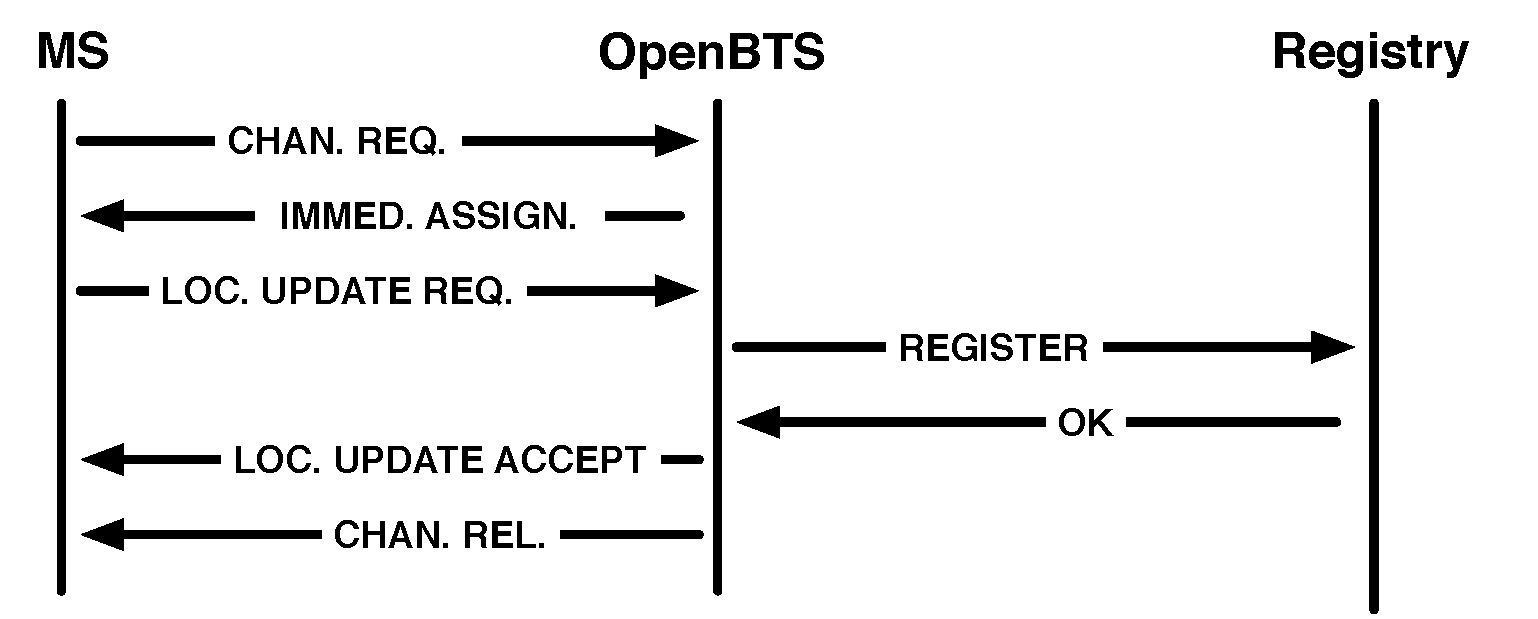
\includegraphics[width=6in]{LURLadder.pdf}
\caption{GSM location update mapped to a SIP REGISTER (non-authenticating case).}
\label{fig:LURLadder}
\end{center}
\end{figure}



\subsection{Call Control}
Figures \ref{fig:MTCLadder} and \ref{fig:MOCLadder} show the mobile-originated and mobile-terminated call setup cases, using very early assignment for simplicity.  In both cases, once the channel is established, the transaction ladder is essentially that of a SIP-ISDN gateway.

\begin{figure}[htbp]
\begin{center}
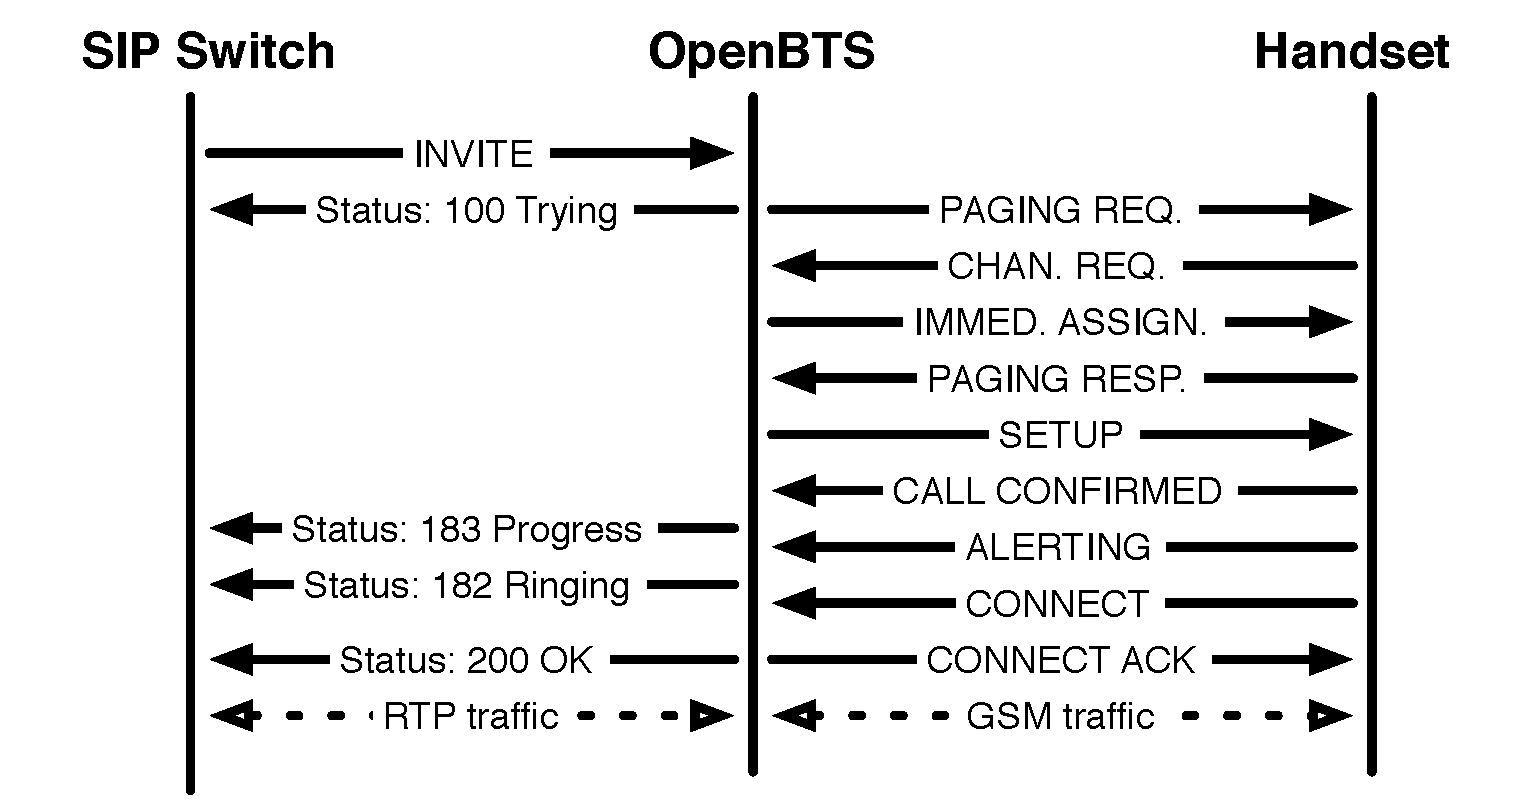
\includegraphics[width=6in]{MTCLadder.pdf}
\caption{A GSM-SIP mobile-terminated call, VEA, normal case.}
\label{fig:MTCLadder}
\end{center}
\end{figure}

\begin{figure}[htbp]
\begin{center}
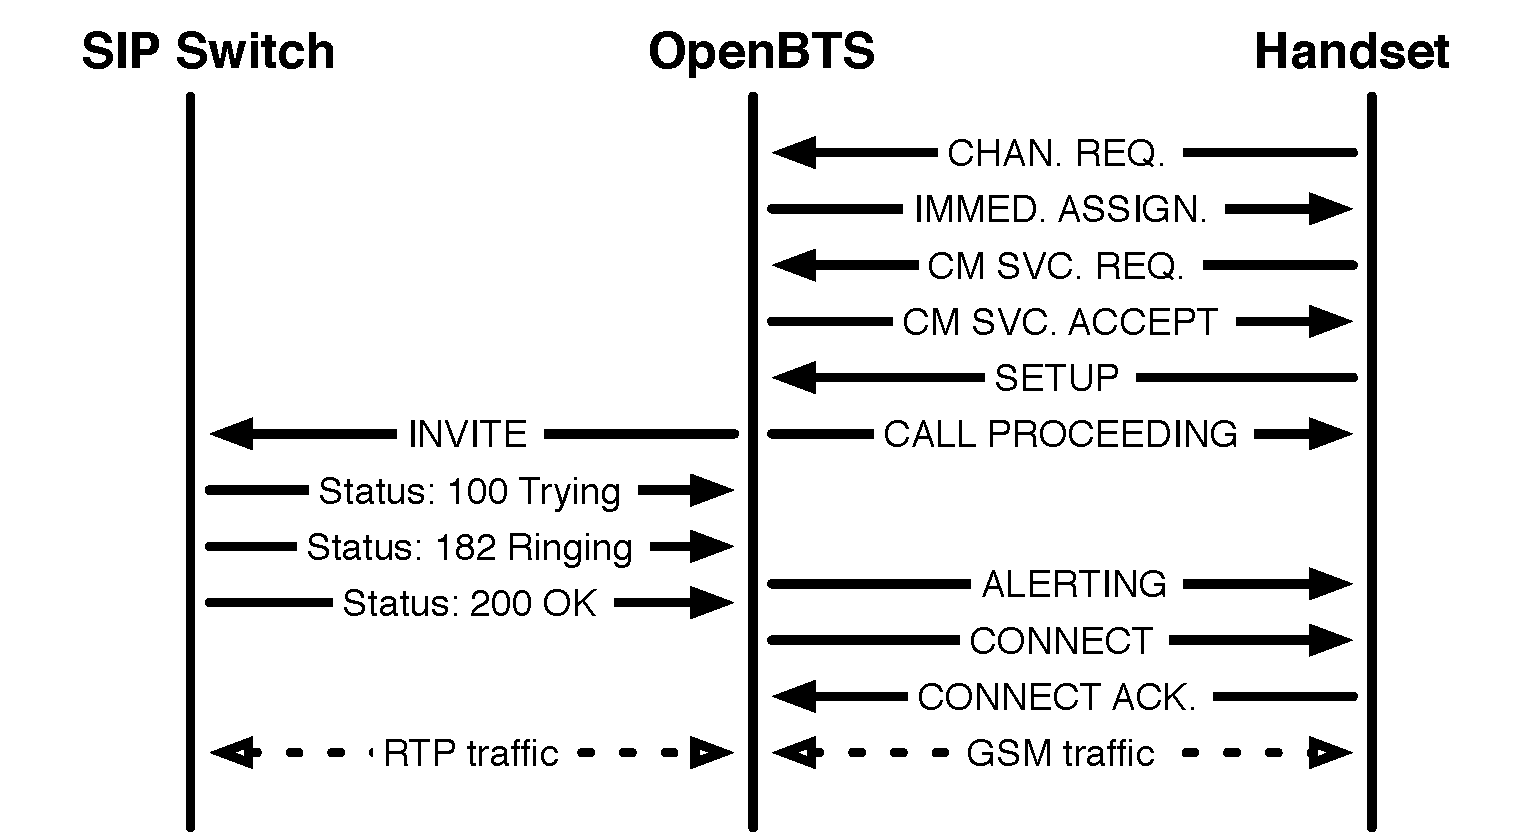
\includegraphics[width=6in]{MOCLadder.pdf}
\caption{A GSM-SIP mobile-originated call, VEA, normal case.}
\label{fig:MOCLadder}
\end{center}
\end{figure}







\chapter{SMS Text Messaging}
\label{chap:smqueue}
GSM text messaging (``short message service'' or SMS) is a service akin to e-mail.
Users can send and receive 140-byte messages, allowing up to 160 characters using the SMS 7-bit alphabet.
Addresses can be ISDN private network, E.164 or e-mail.
SMS is a store-and-forward medium and can be held for minutes, hours or even days if the receiving party is not available.
Text messaging also uses reliable channels, like the SDCCH, with frame retransmission and acknowledgement in L2, making it tolerant of frame erasure rates in excess of 50\%.
These properties make SMS a usable medium over much larger coverage areas than speech, in areas where coverage is spotty or weak and where speech quality would be too poor and calls would disconnect too frequently to be useful.

\section{Internet Messaging Protocols}
For OpenBTS to handle SMS in a manner consistent with its design goals, the GSM SMS protocol must be translated to and from some open protocol from the internet world.
There are many such protocols, but few are well-suited to SMS.

\subsection{The ``Session'' Problem}
Most messaging protocols in the IETF/IP world, like XMPP, are built around the notion of a ``connected session'', a virtual circuit similar the virtual connection of RTP or TCP/IP.  This model assumes an ``always-on'' network connection where the maintenance of the circuit, with occasional keep-alive messages, is cheap and reasonable.

GSM SMS is different.  Maintaining the channel is expensive. There is no keep-alive message mechanism.  The circuit switched connection is created and destroyed with every transfer in a process that can take hundreds of milliseconds.  Each message transfer is an independent transaction.  There is no natural notion of a session.

\subsection{RFC-3428}
RFC-3428 is an IETF standard for the transfer of short messages over the internet.
Among IETF/IP protocols for messaging, RFC-3428 is special in that it supports ``page mode'' messaging, without any notion of a session; there is no INVITE to start the transaction or BYE to end it.  This makes it a natural fit for SMS.  RFC-3428 is straightforward.  The sending entity sends a SIP MESSAGE method to the intended receiver.  The receiver gives one of the standard SIP responses, preferably 200 OK or 202 Queued to indicate a successful transfer, or a 4xx or 5xx response to indicate failure.


\section{Smqueue}
The delivery of each text message depends on a store-and-forward facility in the network.
Smqueue provides this facility.
In the P2.8 release, smqueue is provided with source code under GPLv3.%
\footnote{This will not be true in future releases.}

\subsection{Design and Operation of Smqueue}
The core of smqueue is a queue of messages awaiting delivery.  Messages wait in this queue, potentially through multiple delivery attempts, until delivery is confirmed or until the message is determined to be undeliverable.  The operation is similar to that of an email server.

\subsection{Addressing in Smqueue}
Smqueue recognizes two kinds of addresses: ISDN/E.164 numeric addresses and SIP usernames.  Any all-numeric address is assumed to be an ISDN/E.164 address and smqueue will attempt to resolve it to a SIP username using the subscriber registry.  Any address that is not all-numeric is assumed to be a SIP username in the operator's network.


\subsection{Configuration of Smqueue}
Smqueue is configured through an sqlite3 database table using the same schema as the OpenBTS configuration table.
As of release P2.8, the configuration can be changed only by restarting smqueue after changing the database.  Some configuration parameters of note are:
\begin{itemize}
	\item Log.Level, Log.Level.* -- These are logging controls that behave the same as those in OpenBTS.config.  See Section~\ref{sec:Logging} for more information.
	\item SIP.myIP -- The IP address of the smqueue machine as seen by the subscriber registry server.
	\item SIP.myIP2 -- The IP address of the smqueue machine as seen by remote gateways.
	\item SIP.global\_relay -- The IP address of a remote RFC-3428 server for delivery of non-local messages.  If no such gateway is available, this parameter should be an empty string ('').  This parameter can be used to build a hierarchy of smqueue servers for large networks.
	\item BounceMessage.* -- A set of error messages sent back to MSs when submitted messages are undeliverable.
	\item SC.* -- Configuration parameters for specific short code functions, not for smqueue itself.  See Section~\ref{sec:shortCodes}.
\end{itemize}

\section{Text Messaging in GSM}
GSM 04.11 and 03.40 define conventional SMS in five layers:
\begin{enumerate}
	\item L1 is taken from the Dm channel type used, either SDCCH or SACCH. This layer terminates in the BSC.
	\item L2 is normally LAPDm. This layer terminates in the BTS.
	\item L3, the connection layer, is defined in GSM 04.11 Section 5. This layer terminates in the MSC.
	\item L4, the relay layer, is defined in GSM 04.11 Section 6. This layer terminates in the MSC.
	\item L5, the transfer layer, is defined in GSM 03.40. This layer terminates in the SMSC.
\end{enumerate}
As a general rule, every message transferred in L(n) requires both a transfer and an acknowledgment on L(n-1).

In the OpenBTS realization of SMS, there is no MSC, so L3 terminates in OpenBTS and L4 is a SIP relay to smqueue, which takes the place of the SMSC.

\subsection{Layers of SMS in OpenBTS and Smqueue}
We will now consider the handling of each layer of SMS by OpenBTS and smqueue.

\subsubsection{SMS in L3}
The Um L3 part of SMS uses three messages:
\begin{itemize}
	\item CP-DATA to transfer an RPDU across Um and into L4.
	\item CP-ACK to acknowledge the transfer of an RPDU across Um and into L4.
	\item CP-ERROR to report the failure to transfer an RPDU to L4.
\end{itemize}
An RPDU is a ``relay (layer) protocol data unit'', which is just an encapsulation of a message from L4.
The operation in L3 is simple.  The entity that needs to transfer an RPDU sends it in a CP-DATA message.  The receiving entity responds with CP-ACK or CP-ERROR.  Transactions are non-overlapping.

The action of OpenBTS upon receiving CP-DATA from an MS is to verify the correct encoding of the L3 part of the message and respond with CP-ACK or CP-ERROR.
OpenBTS then extracts the RPDU, transfers it to smqueue as an application/vnd.3gpp.sms MIME payload in a SIP MESSAGE method and waits for a response (200 OK or 202 Queued for success or 4xx or timeout for failure).

After sending CP-DATA to an MS, OpenBTS waits for CP-ACK or CP-ERROR, proceeding after CP-ACK or aborting the transaction after CP-ERROR.

\subsubsection{SMS in L4}
The Um L4 part of SMS uses four messages:
\begin{itemize}
	\item RP-DATA to transfer a TPDU across Um and into L5.
	\item RP-ACK to acknowledge the transfer of a TPDU across Um and into L5.
	\item RP-ERROR to report the failure to transfer an TPDU to L5.
	\item RP-SMMA for the MS to report that it has more memory available to receive SMS messages (not supported by OpenBTS~P2.8).
\end{itemize}
An TPDU is a ``transfer (layer) protocol data unit'', which is just an encapsulation of a message from L5.
OpenBTS translates between SIP and SMS L4 as follows:
\begin{itemize}
	\item RP-DATA -- MESSAGE method with the RPDU as an application/vnd.3gpp.sms MIME payload
	\item RP-ACK -- 200 OK or 202 Queued response
	\item RP-ERROR -- any other response or timeout
	\item RP-SMMA -- not supported in P2.8
\end{itemize}

\subsubsection{SMS in L5}
The Um L5 part of SMS uses these message:
\begin{itemize}
	\item SMS-SUBMIT to transfer a text message from the MS to the network.
	\item SMS-DELIVER to transfer a text message from the network to the MS.
\end{itemize}
OpenBTS transfers L5 PDUs (TPDUs) as opaque payloads. Smqueue manipulates L5 headers as needed to convert SMS-SUMBIT TPDUs into SMS-DELIVER TPDUs during the delivery process.


\subsection{RFC-3428/SMS Transaction Ladders}
Now we take a look at all of the GSM layers and the SIP transactions together.%
\footnote{Strictly speaking, page-mode message transfers are not transactions in SIP, since they are not contained within an INVITE-BYE session.  However, these transfers \emph{are} transactions inside of OpenBTS and will be referred to as transactions throughout the OpenBTS documentation.}

\subsubsection{Mobile Terminated SMS}
Figure~\ref{fig:MTSMSLadder} shows a complete mobile terminated SMS transfer, where the network, through smqueue, transfers a text message to the MS.  The message arrives at smqueue from the outside world addressed either to a SIP user or to a numeric address.  Smqueue resolves the destination address to an IMSI-based SIP user name and forwards the message to OpenBTS.  OpenBTS pages the MS, establishes a channel, transfers the message as SMS and then responds to smqueue with 200 OK.

The most common failure in the mobile terminated transfer is that the MS does not respond to paging.  In this case, smqueue never receives any response.  The message remains in the smqueue delivery queue and another delivery attempt will be made in a few minutes.

\begin{figure}[htbp]
\begin{center}
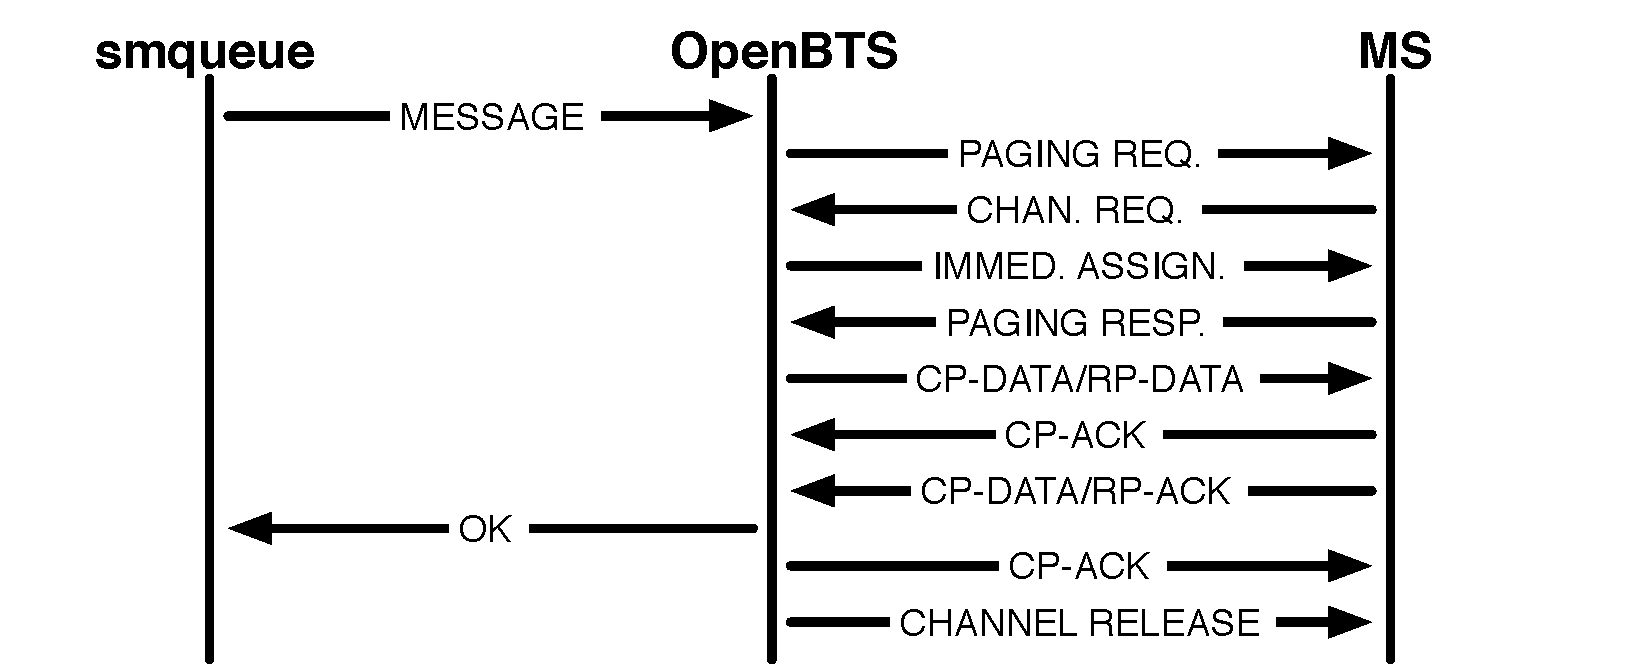
\includegraphics[width=6in]{MTSMSLadder.pdf}
\caption{Mobile-terminated SMS transfer with no parallel call, normal case.}
\label{fig:MTSMSLadder}
\end{center}
\end{figure}

\subsubsection{Mobile Originated SMS}
Figure~\ref{fig:MOSMSLadder} shows a complete mobile originated SMS transfer, where the MS, transfers a text message to smqueue for later delivery to its addressee.  The message originates in the MS with a numeric address.  The MS establishes a radio channel to OpenBTS and then sends the text message TPDU in an RP-DATA message.  OpenBTS translates the TPDU to a SIP MESSAGE method and sends that to smqueue.  Smqueue responds with OK and then OpenBTS responds to the MS with RP-ACK.

\begin{figure}[htbp]
\begin{center}
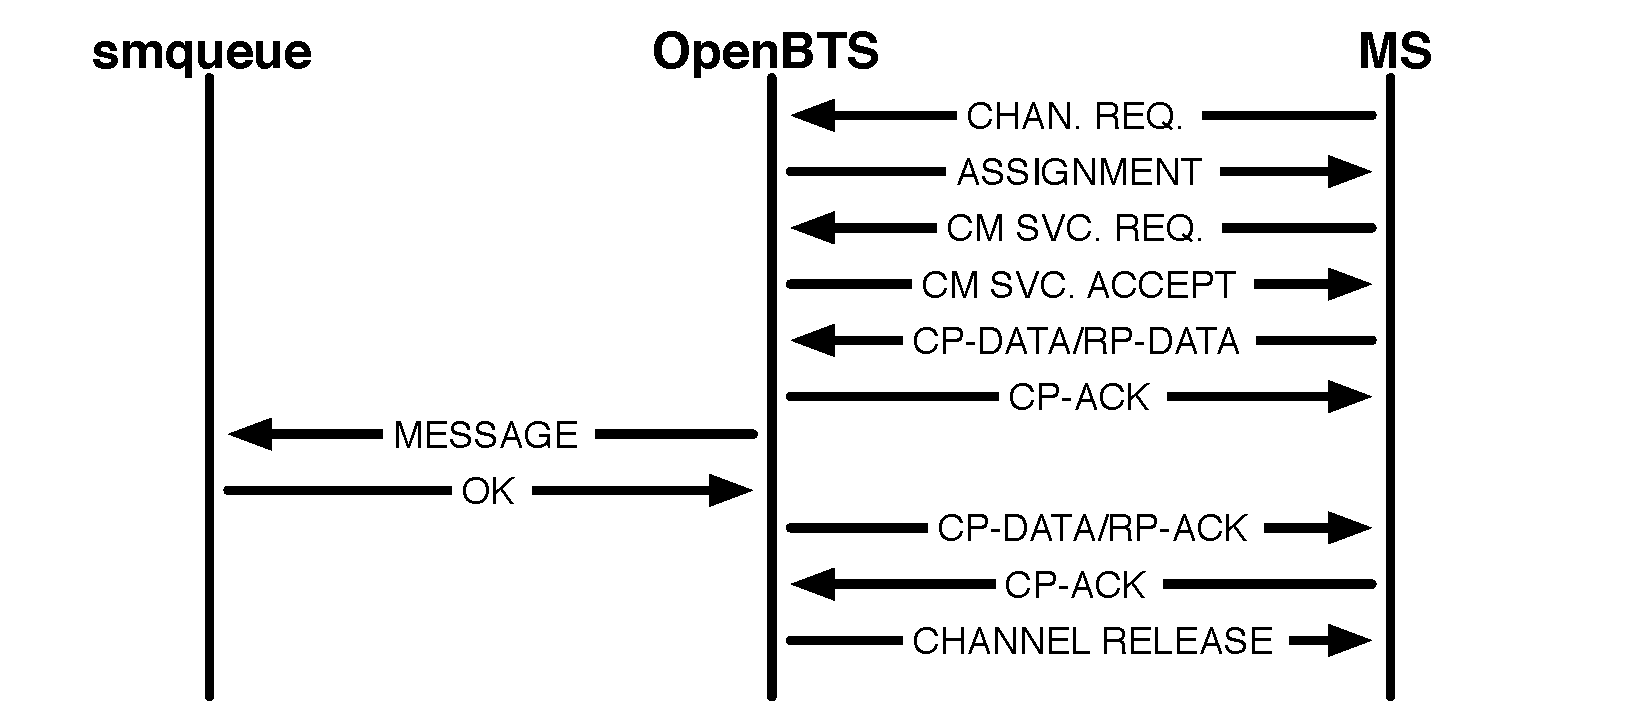
\includegraphics[width=6in]{MOSMSLadder.pdf}
\caption{Mobile-originated SMS transfer with no parallel call, normal case.}
\label{fig:MOSMSLadder}
\end{center}
\end{figure}


\section{Short Code Applications}
\label{sec:shortCodes}
Short codes are local addresses within smqueue that terminate in local application code.  A message sent to a short code becomes an input argument to a short code handler function, instead of being delivered to another user. Short code functions provide a means of writing interactive applications based on text messaging.
A typical SMS-based application would normal comprise several short code addresses and handlers sharing common data.

\subsection{Short Code Implementation}
The short code implementation in OpenBTS~P2.8 is primitive but functional.  Each short code handler is a C++ function coded directly into smqueue/smcommands.cpp.%
\footnote{In future releases, short codes will be implemented as external modules, not directly in smqueue.  However, the calling interface will be maintained to allow reuse of legacy short code source code in these nodules.}
The arguments to a short code handler are the source IMSI of the message, the message text and a short\_code\_params data structure into which any reply message can be written.  The return value from a short code handler is a status code called short\_code\_action.  See smqueue/smcommands.cpp for examples.%

Once a short code handler function is defined, it must also be registered at a numeric address.  This happens in SMqueue::init\_smcommands(), also defined in smqueue/smcommands.cpp.

\subsection{Existing Short Code Applications}
\label{sec:existingShortCodes}
There are a few interesting short code applications built in to the standard release of smqueue, although they are all simple applications each requiring only a single handler function.
Not all short codes are documented here.  Undocumented short codes are left disabled in the default configuration. Refer to the smcommands.cpp source code for information on undocumented short codes.
To disable any short code function, set its short code address to null in the configuration table.

\subsubsection{Autoprovisioning (``Register'')}
\label{sec:autoprovisioning}
The autoprovisioning application allows OpenBTS users to create new entries in the subscriber registry  via SMS.  The user sends his desired telephone number in a text message to the autoprovisioning short code address.  If the requested number has an acceptable number of digits and is not already assigned to a user, the autoprovisioning handler function will perform the steps described in Section~\ref{sec:SMSProvisioning} to provision the new user into the subscriber registry.  The autoprovisioning short code handler function is called shortcode\_register and it is configured through the SC.Register.* parameters in the smqueue configuration table.

For autoprovisioning to work, OpenBTS must also be configured with open registration enabled so that unprovisioned MSs will show service and be capable of sending text messages.  The open registration welcome message can be a powerful way to advertise this feature, especially if the return short code of the welcome message is the same as the short code of the autoprovisioning function.  See Section~\ref{sec:openRegistration} for more information.

\subsubsection{Email}
Any text message send to this address is expected to start with an internet email address.  The short code function forwards the message text to that email address using the Unix sendmail utility.

\subsubsection{Info}
This short code handler generates a brief report of smqueue status, returned in a text message.  The implementing function is called shortcode\_four\_one\_one. This short code handler can be configured with the  SC.Info.* parameters.
\subsubsection{Whiplash Quit}
The whiplash\_quit shortcode handler shuts down smqueue if the correct passphrase is sent to the correct address.  This function is useful for development, but should be disabled in deployed systems.   This short code handler can be configured with the  SC.WhiplashQuit.* parameters.

\subsubsection{Zap Queued}
The shortcode\_zap\_queued handler can delete a message with a specific hash tag or can delete all messages in the queue older than 5000 seconds.  This short code application requires a password.  This short code handler can be configured with the  SC.ZapQueued.* parameters in the smqueue configuration table.














\chapter{Other GSM Services}
\label{chap:otherServices}
This chapter covers 2G GSM services beyond speech and SMS text messaging.


\section{Radio Resource Location Protocol (RRLP)}
RRLP is the protocol used between the network and MS to manage location services (LCS).
All handsets sold in the US market are required, under E911 regulations, to include LCS support.
At least 90\% of handsets in use in the US and EU today support this protocol.

The GSM specifications (02.71, 03.71, 04.30, 04.31 and others) define several possible techniques for determining the location of an MS, but by far the most commonly used is assisted GPS (AGPS) and nearly every handset that supports RRLP also supports the AGPS mode.
GPS is the well-known satellite-based positioning system and AGPS-capable handsets include GPS receivers.

\subsection{The Need for Assistance}
Calculation of a position from GPS measurements requires the following information:
\begin{itemize}
	\item Pseduoranges.  These are timing measurements made on the GPS signal.  They are called pseudoranges because they are directly related to the distances from the GPS satellites.  Pseudoranges are derived from signal delay measurements called ``codephases''.
	\item Ephemerides.  These are detailed descriptions of the current satellite orbits, used to calculate the exact location of each satellite in space.
	\item Ionospheric model.  The radio propagation delay through the ionosphere can vary by hundreds or even thousands of nanoseconds and so must be corrected in the positioning calculations to prevent errors of hundreds of meters in the final positioning results.
	\item Seed position.  The GPS positioning signal (the ``C/A code'') has a period of 1~ms, corresponding to a distance of about 300~km.  This means that there are \emph{many} potential solutions for the GPS positioning equations in an irregular lattice around the Earth.  If the GPS receiver does not know its true position within about 200~km, it must check all of these potential solutions in a brute force search before making a reliable position estimate, a process that can take 20 minutes or longer.  To avoid this delay, the GPS receiver requires a seed position within 200~km of its true location.
	\item Rough current time. Current time must be known to within a few seconds to make rough estimates of satellite position and bootstrap the positioning calculations.  Like seed position, rough time can determined through a brute-force search, but that is very time-consuming.
\end{itemize}
In normal GPS operation, the pseudoranges are measured directly from the GPS signal, the ephemerides and ionospheric model are encoded into the GPS signal and the seed position is taken from the most recent successful positioning attempt (usually saved in non-volatile memory between power-cycles).
Often, though, the GPS receiver in a cellular handset has no useful seed position saved and receives the GPS signal too poorly to decode the critical data that is encoded in them.  However, even under these conditions, the GPS receiver can often measure pseudoranges and ``could'' estimate a position if the other information were provided to it through some other channel.  The process of providing this other information is called ``assistance'' or ``aiding'', hence the terms ``assisted GPS'' and ``aiding information''.

The RRLP specification defines two basic modes of operation:
\begin{enumerate}
	\item MS-based, where the network provides ephemeris and ionospheric parameters, rough time and seed position and the GPS receiver in the MS performs the positioning calculation and
	\item network-based, where network provides rough codephases to the MS to bootstrap the measurement process, the MS makes actual codephase measurements, the MS reports the raw codephases back to the network and the network performs the positioning calculation.
\end{enumerate}
OpenBTS P2.8 supports only the MS-based RRLP mode.%
\footnote{Future versions of OpenBTS will support network-based positioning as well.}

\subsection{The RRLP Server}
\subsubsection{Overall Design}
In keeping with the OpenBTS design philosophy, RRLP is not implemented inside OpenBTS, but in an external server that communicates with OpenBTS through an HTTP interface at the L3/L4 boundary.
The role of OpenBTS is to transfer L4 RRLP APDUs between the MS and the RRLP server.
From OpenBTS to the server, these APDUs are encoded in the URLs of HTTP requests.
From the server to OpenBTS, APDUs are passed in HTTP responses.
The RRLP server can be run in each BTS unit, in each cell site or from a single central location.

Because the RRLP server is HTTP based, its actual implementation is as a CGI program in a standard web server.

\subsubsection{Source of Aiding Information}
The primary function of the RRLP server in network-assisted positioning is to provide aiding information.
The RRLP server acquires the current GPS almanac and ephemerides for aiding information from publicly available sources on the internet.%
\footnote{Future versions of OpenBTS will support direct connection of GPS receivers to the RRLP server.}
These parameters total about 2~kB and are downloaded every hour.

The AGPS seed location is provided by the BTS unit that submits the HTTP request to the RRLP server.  This location is defined in the RRLP.* configuration parameters listed in Section~\ref{sec:configTable}.

Rough current time comes from the time-of-day clock on the machine running the RRLP server.  The machine running the RRLP server should also be running NTP (network time protocol) to calibrate its time-of-day clock.

\subsection{RRLP Service Controls and Configuration}

\subsubsection{Server Configuration}
All parameters the control the behavior of the RRLP server are given to it in the URL of the service request.
This means that the server itself has no configuration; all of the configuration is in the client side in the OpenBTS configuration table.  See the GSM.RRLP.* configuration parameter set in Section~\ref{sec:configTable} for more information.

\subsubsection{Invoking RRLP}
The following parameters control whether or not all MS are queried for RRLP position information:
\begin{itemize}
	\item Control.LUR.RRLPQuery
	\item Emergency.RRLP
\end{itemize}
See Section~\ref{sec:configTable} for more information.

%RRLP can also be invoked on a per-subscriber basis by setting the RRLP flag in the subscriber registry.

\subsubsection{Getting RRLP Results}
RRLP results are written to the subscriber registry database, to a table called ``RRLP''.
The schema is:
\begin{verbatim}
CREATE TABLE IF NOT EXISTS RRLP (
  id INTEGER PRIMARY KEY, -- integer key
  name VARCHAR(80) not null, -- SIP user name (IMSI)
  latitude real not null, -- WGS84 latitude in degrees
  longitude real not null, -- WGS84 longitude in degrees
  error real not null,  -- circular error estimate in meters
  time text not null -- Unix time of fix
)
\end{verbatim}




\chapter*{Document History}

\begin{table}[htdp]
%\caption{default}
\begin{center}
\begin{tabular}{|c|c|c|c|}
\hline
Date 		& Doc.\ Rev.\ & Changes \\ \hline \hline
19 Sept 2011	& 1	& derived P2.8 manual rev 1 fron C2.8 manual rev 3 \\
\hline
28 Feb 2012	& 2	& updated cover logo and changed font  \\
\hline
28 June 2013   & 3 & changed the license to CC BY-SA 3.0 \\
\hline
\end{tabular}
\end{center}
\label{default}
\end{table}%

 \end{document}

 
